\documentclass{article}

\usepackage{amsmath, amssymb}
\usepackage{algorithm, float}
\usepackage{etoolbox}
\usepackage{bm}
\usepackage[english]{babel}
\usepackage{graphicx}
\usepackage[colorinlistoftodos]{todonotes}
\usepackage{enumitem}
\usepackage{algpseudocode}
\usepackage{setspace}
%\usepackage[noend]{algpseudocode}

\usepackage{tikz}


\newcommand\tikzmark[1]{%
  \tikz[remember picture,overlay]\node[inner sep=2pt] (#1) {};}
\newcommand\DrawBox[3][]{%
  \tikz[remember picture,overlay]\draw[#1] ([xshift=-3.5em,yshift=7pt]#2.north west) rectangle (#3.south east);}

\algnewcommand\algorithmicinput{\textbf{Input:}}
\algnewcommand\INPUT{\item[\algorithmicinput]}

\algnewcommand\algorithmicoutput{\textbf{Output:}}
\algnewcommand\OUTPUT{\item[\algorithmicoutput]}

\algnewcommand\algorithmicLet{\textbf{Let:}}
\algnewcommand\LET{\item[\algorithmicLet]}



\usepackage{varwidth}% http://ctan.org/pkg/varwidth

\newcommand\NoThen{\renewcommand\algorithmicthen{}}
\newcommand\ReThen{\renewcommand\algorithmicthen{\textbf{then}}}


\makeatletter
\newcommand{\StatexIndent}[1][3]{%
  \setlength\@tempdima{\algorithmicindent}%
  \Statex\hskip\dimexpr#1\@tempdima\relax}%
  


\makeatletter
\newenvironment{breakablealgorithm}
  {% \begin{breakablealgorithm}
   \begin{center}
     \refstepcounter{algorithm}% New algorithm
     \hrule height.8pt depth0pt \kern2pt% \@fs@pre for \@fs@ruled
     \renewcommand{\caption}[2][\relax]{% Make a new \caption
       {\raggedright\textbf{\ALG@name~\thealgorithm} ##2\par}%
       \ifx\relax##1\relax % #1 is \relax
         \addcontentsline{loa}{algorithm}{\protect\numberline{\thealgorithm}##2}%
       \else % #1 is not \relax
         \addcontentsline{loa}{algorithm}{\protect\numberline{\thealgorithm}##1}%
       \fi
       \kern2pt\hrule\kern2pt
     }
  }{% \end{breakablealgorithm}
     \kern2pt\hrule\relax% \@fs@post for \@fs@ruled
   \end{center}
  }


\makeatletter
\AfterEndEnvironment{breakablealgorithm}{\let\@algcomment\relax}
\AtEndEnvironment{breakablealgorithm}{\kern2pt\hrule\relax\vskip3pt\@algcomment}
\let\@algcomment\relax
\newcommand\algcomment[1]{\def\@algcomment{\begin{flushleft}\footnotesize#1\end{flushleft}}}

\makeatother







\iffalse

\errorcontextlines\maxdimen

% begin vertical rule patch for algorithmicx (http://tex.stackexchange.com/questions/144840/vertical-loop-block-lines-in-algorithmicx-with-noend-option)
\makeatletter
% start with some helper code
% This is the vertical rule that is inserted
\newcommand*{\algrule}[1][\algorithmicindent]{\makebox[#1][l]{\hspace*{.5em}\vrule height .75\baselineskip depth .25\baselineskip}}%

\newcount\ALG@printindent@tempcnta
\def\ALG@printindent{%
    \ifnum \theALG@nested>0% is there anything to print
        \ifx\ALG@text\ALG@x@notext% is this an end group without any text?
            % do nothing
            \addvspace{-3pt}% FUDGE for cases where no text is shown, to make the rules line up
        \else
            \unskip
            % draw a rule for each indent level
            \ALG@printindent@tempcnta=1
            \loop
                \algrule[\csname ALG@ind@\the\ALG@printindent@tempcnta\endcsname]%
                \advance \ALG@printindent@tempcnta 1
            \ifnum \ALG@printindent@tempcnta<\numexpr\theALG@nested+1\relax% can't do <=, so add one to RHS and use < instead
            \repeat
        \fi
    \fi
    }%
% the following line injects our new indent handling code in place of the default spacing
\patchcmd{\ALG@doentity}{\noindent\hskip\ALG@tlm}{\ALG@printindent}{}{\errmessage{failed to patch}}
\makeatother

\fi

\def\NoNumber#1{{\def\alglinenumber##1{}\State #1}\addtocounter{ALG@line}{-1}}
%\def\NoNumberb#1{\def\alglinenumber##1{}\State #1\addtocounter{ALG@line}{-1}}




\begin{document}

\documentclass[A4, 11pt, preprint]{elsarticle}

%\usepackage{cite}

\usepackage[fleqn]{amsmath}
\usepackage{amssymb}
\usepackage{algorithm}
\usepackage{algpseudocode}
\usepackage{etoolbox}
\usepackage{setspace}
\usepackage{lineno,hyperref}


\makeatletter
\AfterEndEnvironment{algorithm}{\let\@algcomment\relax}
\AtEndEnvironment{algorithm}{\kern2pt\hrule\relax\vskip3pt\@algcomment}
\let\@algcomment\relax
\newcommand\algcomment[1]{\def\@algcomment{\footnotesize#1}}


\renewcommand\fs@ruled{\def\@fs@cfont{\bfseries}\let\@fs@capt\floatc@ruled
  \def\@fs@pre{\hrule height.8pt depth0pt \kern2pt}%
  \def\@fs@post{}%
  \def\@fs@mid{\kern2pt\hrule\kern2pt}%
  \let\@fs@iftopcapt\iftrue}
\makeatother


\makeatletter
\g@addto@macro{\endtabular}{\rowfont{}}% Clear row font
\makeatother
\newcommand{\rowfonttype}{}% Current row font
\newcommand{\rowfont}[1]{% Set current row font
   \gdef\rowfonttype{#1}#1%
}


\usepackage{array}

\usepackage{booktabs}

\newcolumntype{P}[1]{>{\centering\arraybackslash}p{#1}}

\usepackage{stfloats}

\usepackage{url}

\usepackage{graphicx}

\usepackage{multicol}

\usepackage{caption}
\usepackage{subcaption}

\usepackage{siunitx}

\usepackage[hang,flushmargin]{footmisc}

%\usepackage{auto-pst-pdf}

\usepackage{multirow}
\usepackage{array}
\usepackage{tabu}

\captionsetup{font=footnotesize}


\newcommand{\tcent}[1]{\multicolumn{1}{c|}{#1}}


%%%%%%%%% DRAWING %%%%%%%%%


\usepackage{bera}
\usepackage{pstricks}
\usepackage[T1]{fontenc}
\usepackage{epsfig}
\usepackage{pst-grad} % For gradients
\usepackage{pst-plot} % For axes
\usepackage[space]{grffile} % For spaces in paths
\usepackage{etoolbox} % For spaces in paths
\usepackage{pst-node,pst-blur,pstricks-add}
\usepackage[utf8]{inputenc}

\usepackage{bm}



%%%%%%%%%%%%%%%%%%%%%%%%%%%%%%%%%%%%%%%%




\newcommand{\fnt}[1]{\fontsize{#1}{#1}\selectfont}
\newcommand{\fntt}{\fnt{7}}


\newcommand{\bbfamily}{\fontencoding{U}\fontfamily{bbold}\selectfont}
\DeclareMathAlphabet{\mathbbold}{U}{bbold}{m}{n}

\makeatletter
\renewcommand{\ALG@beginalgorithmic}{\fnt{8}}
\makeatother

\newcommand\numberthis{\addtocounter{equation}{1}\tag{\theequation}}


% correct bad hyphenation here
\hyphenation{op-tical net-works semi-conduc-tor}


\newcolumntype{?}{!{\vrule width 1pt}}



\iffalse

\usepackage{fancyhdr}

\pagestyle{fancy}
\newcommand\shorttitle{{\fontfamily{zlmtt}\selectfont\fnt{9} Improvements on Biased Random-Key Genetic Algorithms \\ for Non-Linearly Constrained Global Optimization}}
\newcommand\authors{{\fontfamily{zlmtt}\selectfont\fnt{9} M. P. Ferreira, M. L. Rocha, A. J. Silva Neto}}
\fancyhf{}
\renewcommand\headrulewidth{0pt}
\fancyhead[C]{%
\ifodd\value{page}
  \small\scshape\authors
\else
  \small\scshape\shorttitle
\fi }

\fancyhead[R]{\thepage\ifodd\value{page}\else\hfill\fi}


\makeatletter
\def\blfootnote{\gdef\@thefnmark{}\@footnotetext}
\makeatother

\fi



\captionsetup[algorithm]{format=hang,singlelinecheck=false}

%\renewcommand{\thesection}{\arabic{section}} 
%\renewcommand{\thesubsection}{\thesection.\arabic{subsection}}




% ALGORITHMS

\usepackage{tikz}


\newcommand\tikzmark[1]{%
  \tikz[remember picture,overlay]\node[inner sep=2pt] (#1) {};}
\newcommand\DrawBox[3][]{%
  \tikz[remember picture,overlay]\draw[#1] ([xshift=-3.5em,yshift=7pt]#2.north west) rectangle (#3.south east);}

\algnewcommand\algorithmicinput{\textbf{Input:}}
\algnewcommand\INPUT{\item[\algorithmicinput]}

\algnewcommand\algorithmicoutput{\textbf{Output:}}
\algnewcommand\OUTPUT{\item[\algorithmicoutput]}

\algnewcommand\algorithmicLet{\textbf{Let:}}
\algnewcommand\LET{\item[\algorithmicLet]}



\usepackage{varwidth}% http://ctan.org/pkg/varwidth

\newcommand\NoThen{\renewcommand\algorithmicthen{}}
\newcommand\ReThen{\renewcommand\algorithmicthen{\textbf{then}}}


\makeatletter
\newcommand{\StatexIndent}[1][3]{%
  \setlength\@tempdima{\algorithmicindent}%
  \Statex\hskip\dimexpr#1\@tempdima\relax}%
  


\makeatletter
\newenvironment{breakablealgorithm}
  {% \begin{breakablealgorithm}
   \begin{center}
     \refstepcounter{algorithm}% New algorithm
     \hrule height.8pt depth0pt \kern2pt% \@fs@pre for \@fs@ruled
     \renewcommand{\caption}[2][\relax]{% Make a new \caption
       {\raggedright\textbf{\ALG@name~\thealgorithm} ##2\par}%
       \ifx\relax##1\relax % #1 is \relax
         \addcontentsline{loa}{algorithm}{\protect\numberline{\thealgorithm}##2}%
       \else % #1 is not \relax
         \addcontentsline{loa}{algorithm}{\protect\numberline{\thealgorithm}##1}%
       \fi
       \kern2pt\hrule\kern2pt
     }
  }{% \end{breakablealgorithm}
     \kern2pt\hrule\relax% \@fs@post for \@fs@ruled
   \end{center}
  }


\algtext*{EndWhile}% Remove "end while" text
\algtext*{EndIf}% Remove "end if" text
\algtext*{EndFor}% Remove "end if" text


%%%%%%%%%%%%%%%%%%%%%%%
%% Elsevier bibliography styles
%%%%%%%%%%%%%%%%%%%%%%%
%% To change the style, put a % in front of the second line of the current style and
%% remove the % from the second line of the style you would like to use.
%%%%%%%%%%%%%%%%%%%%%%%

%% Numbered
%\bibliographystyle{model1-num-names}

%% Numbered without titles
%\bibliographystyle{model1a-num-names}

%% Harvard
%\bibliographystyle{model2-names.bst}\biboptions{authoryear}

%% Vancouver numbered
%\usepackage{numcompress}\bibliographystyle{model3-num-names}

%% Vancouver name/year
%\usepackage{numcompress}\bibliographystyle{model4-names}\biboptions{authoryear}

%% APA style
\bibliographystyle{src/BibStyle/model5-names}\biboptions{authoryear}

%% AMA style
%\usepackage{numcompress}\bibliographystyle{model6-num-names}

%% `Elsevier LaTeX' style
%\bibliographystyle{elsarticle-num}
%%%%%%%%%%%%%%%%%%%%%%%



\modulolinenumbers[5]

\journal{Expert Systems with Applications}

\onehalfspacing





\begin{document}



\begin{frontmatter}

\title{A Constrained Iterative Topographical Global \\ Optimization Applied to Engineering Optimization}

%\tnotetext[mytitlenote]{Fully documented templates are available in the elsarticle package on \href{http://www.ctan.org/tex-archive/macros/latex/contrib/elsarticle}{CTAN}.}


%% Group authors per affiliation:
%\author{Elsevier\fnref{footUFT}}
%\address{Radarweg 29, Amsterdam}
%\fntext[footUFT]{Universidade Federal do Tocantins}


\author[label1]{Matheus~Pedroza~Ferreira}
\ead{matheuspedrozaferreira@uft.edu.br}

\author[label1]{Marcelo~Lisboa~Rocha\corref{cor1}}
\ead{mlisboa@uft.edu.br}

\author[label2]{Ant\^onio~J.~Silva~Neto}
\ead{ajsneto@iprj.uerj.br}

\author[label3]{Wagner~F.~Sacco}
\ead{wagner.sacco@ufopa.edu.br}



\address[label1]{Departamento de Ci\^encia da Computa\c{c}\~ao, Universidade Federal do Tocantins, Quadra 109 Norte, Avenida NS-15, ALCNO-14, Palmas, Tocantins, Brazil}

\address[label2]{Departamento de Engenharia Mec\^anica e Energia, Instituto Polit\'ecnico, Universidade do Estado do Rio de Janeiro IPRJ/UERJ, RJ, Brazil}

\address[label3]{Instituto de Engenharia e Geociências, Universidade Federal do Oeste do Pará, PA, Brazil}



\cortext[cor1]{Corresponding authors}










\iffalse

\fntext[footMat]{Dept. de Ci\^encia da Computa\c{c}\~ao, Universidade Federal do Tocantins. \\ \textit{E-mail}: \textbf{matheuspedrozaferreira@uft.edu.br}}

\fntext[footLis]{Dept. de Ci\^encia da Computa\c{c}\~ao, Universidade Federal do Tocantins. \\ \textit{E-mail}: \textbf{mlisboa@uft.edu.br}}

\fntext[footAnt]{Departamento de Engenharia Mec\^anica e Energia, Instituto Politécnico, Universidade do Estado do Rio de Janeiro IPRJ/UERJ. \\ \textit{E-mail}: \textbf{ajsneto@iprj.uerj.br}}

\fi





%% or include affiliations in footnotes:
%\author[mymainaddress,mysecondaryaddress]{Elsevier Inc}
%\ead[url]{www.elsevier.com}

%\author[mysecondaryaddress]{Global Customer Service\corref{mycorrespondingauthor}}
%\cortext[mycorrespondingauthor]{Corresponding author}
%\ead{support@elsevier.com}



\begin{abstract}
    Nonlinear optimization is an active line of research, given the wide range of scientific fields that benefit from its development. In the last years, the meta-heuristics proved to be one of the most effective methods to tackle difficult optimization problems, providing an alternative in cases where exact methods would be unfeasible. In this work, we developed a method based on the Iterative Topographical Global Optimization meta-heuristic, which we call C-ITGO, incorporating specific mechanisms to solve nonlinearly constrained optimization problems. We use the method developed in this work to optimize eight complex engineering design problems and compare the results obtained here against several methods found in the literature. In the tests performed, C-ITGO outperforms all competing methods, achieving state of the art results for the problems considered.
\end{abstract}


\begin{keyword}
Meta-heuristics \sep ITGO \sep Optimization \sep Engineering Problems.
\end{keyword}


%\begin{keyword}
%Metaheuristics \sep BRKGA \sep Global Optimization \sep Local Search.
%\MSC[2010] 00-01\sep  99-00
%\end{keyword}


\end{frontmatter}


%\blfootnote{\fnt{9} \textit{Key words.}  Metaheuristics, BRKGA, Global Optimization, Local Search.}




%\linenumbers


\section{Introduction} \label{sec:Introduction}

In recent years, there has been an increase in the interest of applying meta-heuristics to solve difficult numerical optimization problems, mainly due to the impossibility of obtaining good quality solutions to some complex problems using standard local optimization methods. It is usual to find nonlinear constrained real-world problems which are not smooth or not even continuous, ruling out the possibility to apply any gradient-based optimization procedure.

Even when the problem at hand has continuous derivatives, it may be multimodal, having many local optima. Any deterministic local procedure is confined to finding sub-optimal solutions for any multimodal problem of reasonable size. Many modern meta-heuristics, on the other hand, are capable of finding an optimal or nearly optimal solution to these problems within a feasible amount of time.

Along with the meta-heuristics, there exist a class of deterministic global optimization methods that can tackle multimodal optimization problems, assuring convergence to the global optimum with predefined tolerance. These methods are in general more complex than meta-heuristics, having rigorous convergence proofs and requiring certain mathematical background to be correctly understood and implemented \citep{BOOKS1, BOOKS2, NAT}. Some examples include the well known DIRECT (DIviding RECTangles) method \citep{DIRECT}, its locally biased variant \citep{DIRECTL}, the ADC (Adaptive Diagonal Curves) algorithm \citep{ADC}, and some more recent methods \cite{ADC2, GEO, SIMP}. A thorough comparison between meta-heuristics and deterministic global optimization algorithms is made in \cite{NAT}, using some novel methods.

Among the most recent meta-heuristics used to solve nonlinear constrained optimization problems, we can cite some well known methods, such as Particle Swarm Optimization (PSO) \citep{IPSO, IAPSO, PSO1}, Artificial Bee Colony (ABC) \citep{CB-ABC, IABC-Mal}, Differential Evolution (DE) \citep{DE1, DE2, MVDE}, Genetic Algorithms (GA) \citep{GA1} and many other new methods, being some of them nature inspired \citep{CS, WCA, MBA}.

The objective is to find the best solution in a search space that satisfies some criteria, expressed in the form of constraints, whose value is rated according to a function. For minimization, a general nonlinearly constrained optimization problem can be defined as follows: \\[-3em]

\begin{equation}\label{eq:func}
    \begin{aligned}
    \underset{\bm{x}}{\text{\fnt{10} arg\,min}} \ \ & f(\bm{x}) \\
    \text{s.t.} \quad & g_j(\bm{x}) \leq 0, \qquad j = 1, ..., p  \\
                      & h_k(\bm{x}) = 0, \qquad k = 1, ..., q  \\ 
                      & l_i \leq x_i \leq u_i, \qquad i = 1, ..., n 
    \end{aligned}
\end{equation}

\noindent
where $f(\cdot)$ is the objective function or fitness function, $\bm{x} = (x_1, ..., x_n)$ is a solution vector containing $n$ continuous or discrete values, $g_j(\cdot), \ j = 1, ..., p$, and $h_k(\cdot), \ k = 1, ..., q$, are the inequality and equality constraints respectively, where both can be nonlinear. The vectors $\bm{l}$ and $\bm{u}$ define the lower and upper bounds of the solution space. We also define the sum of constraint violation as: \\[-3em]

\begin{equation}\label{eq:viol}
    v(\bm{x}) = \sum_{j=1}^p max\{g_j(\bm{x}), 0\} + \sum_{k=1}^q |h_k(\bm{x})|
\end{equation}

\noindent
so a solution $\bm{x}$ is feasible only when $v(\bm{x}) = 0$. 

In this work, we develop some modifications over a successful meta-heuristic for continuous optimization, known as Iterative Topographical Global Optimization (ITGO) \citep{ITGO0}. The modifications consist of adapting ITGO to work with constrained optimization issues, calling this new algorithm as the Constrained version of ITGO (C-ITGO). We compare the results obtained for eight complex constrained engineering design problems, used as a benchmark against several state-of-the-art methods. We show that C-ITGO outperforms the best competing techniques from literature, mainly relative to the number of function evaluations that characterize the execution effort of the technique.

The structure of the paper is as follows. Section \ref{sec:Methods} presents the C-ITGO method, as well as the details of its implementation and the parameters used in the tests. We compare the developed algorithm against the competing methods in Section \ref{sec:Results} and make the final conclusions in Section \ref{sec:Conclusion}.


\section{The Constrained Topographical Global Optimization Algorithm}\label{sec:Methods}

The TGO algorithm, which stands for \textit{Topographical Global Optimization}, is a meta-heuristic developed by \cite{ITGO1} for solving continuous optimization problems, possibly non-smooth and multimodal. The method has three steps: the random uniform generation of a population of solutions over the domain of the problem, the selection of some of the individuals of the population based on the topography of the function to be optimized, and the application of some sort of local search in the selected elements.


Initially, the TGO creates a population of size $M$ denoted by $P = \{\bm{x}_1, \bm{x}_2, ..., \allowbreak \bm{x}_M\}$, uniformly distributed in the solution space. The TGO performance depends directly on the algorithm used in the generation of the population, and, consequently, on the pseudo-random number generator. In this work, we use the Sobol sequences \cite{Sobol, ITGO3}, which has a significantly more uniform distribution than an excellent pseudo-random number generator. The Fig. \ref{fig:Sobol} shows the distribution of 300 points in the domain $[0, 1]^2$, with 150 of them (blue dots) generated by the pseudo-random generator Mersene Twister proposed by \cite{mt19937}. The other points (red dots) are the 150 first elements of a Sobol sequence. From Fig \ref{fig:Sobol} is possible to observe that the points generated by Sobol sequence cover the space more uniformly than that of Mersene Twister.


\begin{figure*}[h]
\begin{center}
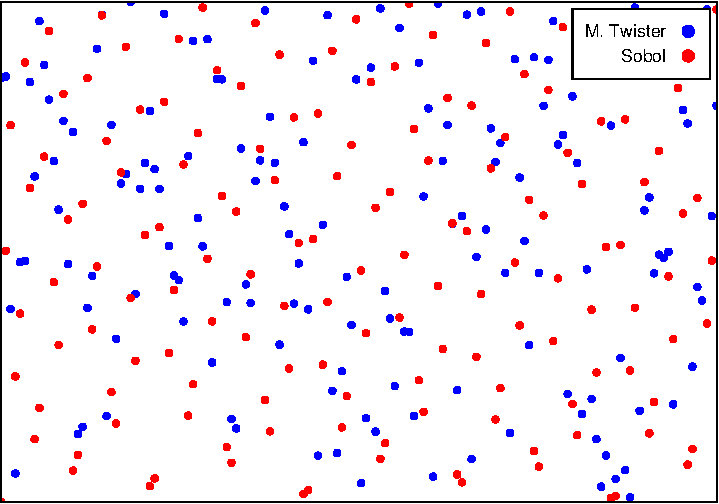
\includegraphics[scale=0.8]{scatter-crop.pdf}
\end{center}
\captionsetup{justification=centering}
\caption{Example showing the distribution of points in the domain $[0, 1]^2$ by the Mersenne Twister generator (blue points) and by a Sobol sequence (red points). }\label{fig:Sobol}
\end{figure*}


The next step is the construction of a graph over possible solutions that incorporate information regarding the topography of the function $f(\cdot)$. Consider now a integer $K > 0$. We define the $KNN_K(\bm{x})$ neighborhood as the set of the $K$ elements of the population $P$, different of $\bm{x}$, that have the smallest euclidean distance from $\bm{x}$.

A directed graph is then defined, having a vertex for every solution in the population. For each individual $\bm{x}$, a directed edge is created pointing to every element $\bm{y}$ of the population $P$ such that $\bm{y} \in KNN_K(\bm{x})$ and $f(\bm{x}) \leq f(\bm{y})$. With this construction, every vertex has at most $K$ edges, being some of them incoming and some outgoing. A topography matrix $A \in \mathbb{R}^{M \times M}$ is created based on this graph, defined as:


\[
    A_{i, j} = 
\begin{cases}
    1,& \text{if } f(\bm{x}_i) \leq f(\bm{x}_j) \ \text{ and } \ \bm{x}_j \in KNN_K(\bm{x}_i) \\
    0,& \text{otherwise}
\end{cases}
\]
\\[-1.5em]


The matrix $A$ tells us if the element $\bm{x}_i$ has better fitness than the element $\bm{x}_j$, given that $\bm{x}_j$ is in the $KNN$ set of $\bm{x}_i$. The graph defined previously has a direct link with the topography matrix: a directed edge between elements $\bm{x}_i$ and $\bm{x}_j$ only exists if $A_{i, j} = 1$. We have then created an ordering of the elements of the population based on the position on space, the objective function value, and the neighborhood defined by $K$.

The topographic heuristic is based on selecting every individual $\bm{x}_i$ such that $\sum_j^M A_{i, j} = K$, that is, every individual that has better fitness than every element of its $KNN$ set. Likewise, every vertex that has $K$ outgoing edges. These elements are considered local optimum points based on the estimated topography of the function $f(\cdot)$.

As there is no guarantee that the individuals selected are really local optimum points (the optimality relationship is based only on the topography created by the individuals of the population), the application of 
some algorithm for fine tuning is necessary.

The last step of the TGO method consists in applying some sort of local search in every local optimum point based on the topographic heuristic. Regarding the local search, many procedures used in the TGO are found in the literature, such as pattern search algorithms \citep{ITGO2}, derivative-based \citep{ITGO3} and derivative-free \citep{ITGO4} optimization methods. The local search algorithm depends directly on the properties of the function to be optimized and is of significative impact in the overall performance of the method.

We consider now a simple example. Let the function $f(\cdot)$ defined by $f(x, y) = sen(x^2) + cos(y^2)$, the population $P$ composed by the 10 elements: \\[-4em]

\begin{equation*}
  \begin{aligned}
& \qquad \bm{x}_1 = (-0.2, 0.16), \qquad \bm{x}_2 = (1.2, -0.3), \qquad \bm{x}_3 = (-0.6, 1.2) \\
& \qquad \bm{x}_4 = (-0.9, 2.4), \qquad \ \, \bm{x}_5 = (2.0, 2.0), \qquad \ \ \ \bm{x}_6 = (2.7, 0.3) \\
& \bm{x}_7 = (0.3, 2.2), \quad \bm{x}_8 = (2.0, -0.2), \quad \bm{x}_9 = (1.3, 2.8), \quad \bm{x}_{10} = (1.3, 1.2) \\
  \end{aligned}
\end{equation*}

\noindent
and the $KNN$ set determined by the $K = 3$ closest neighbors. Fig. \ref{fig:Graph} shows the contour plot of the function and the directed graph created by the population. The topography matrix and the sum of each row are the following:

\[
A=
  \left(\begin{array}{cccccccccc?c}
    1 & 1 & 0 & 0 & 0 & 0 & 0 & 0 & 0 & 1 & \ \bm{3} \\
    0 & 0 & 0 & 0 & 0 & 0 & 0 & 0 & 0 & 0 & \ \bm{0} \\
    0 & 0 & 0 & 0 & 0 & 0 & 0 & 0 & 0 & 0 & \ \bm{0} \\
    0 & 0 & 1 & 0 & 0 & 0 & 0 & 0 & 1 & 0 & \ \bm{2} \\
    0 & 0 & 0 & 0 & 0 & 0 & 1 & 0 & 1 & 1 & \ \bm{3} \\
    0 & 0 & 0 & 0 & 0 & 0 & 0 & 0 & 0 & 1 & \ \bm{1} \\
    0 & 0 & 0 & 1 & 0 & 0 & 0 & 0 & 1 & 0 & \ \bm{2} \\
    0 & 1 & 0 & 0 & 0 & 1 & 0 & 0 & 0 & 1 & \ \bm{3} \\
    0 & 0 & 0 & 0 & 0 & 0 & 0 & 0 & 0 & 0 & \ \bm{0} \\
    0 & 0 & 0 & 0 & 0 & 0 & 0 & 0 & 0 & 0 & \ \bm{0} \\
  \end{array} \right)
\]
\\[-0.5em]

According with the graph and the topography matrix created, it is easy to observe that only the elements $\bm{x}_1$, $\bm{x}_5$ and $\bm{x}_8$ are local optimum, that is, has $K$ outgoing edges and no incoming edge, satisfying $\sum_j^M A_{1, j} = \sum_j^M A_{5, j} = \sum_j^M A_{8, j} = K = 3$.

Even after the application of local search, there is no guarantee that the global optimum was found. It is common to successively apply the TGO method many times, with new elements at each iteration. This procedure is called \textit{ITGO} (\textit{Iterative Topographical Global Optimization}), and consists simply in the iterative application of the TGO method, returning the best element found during all the process.



\begin{figure*}[tp]
\begin{center}
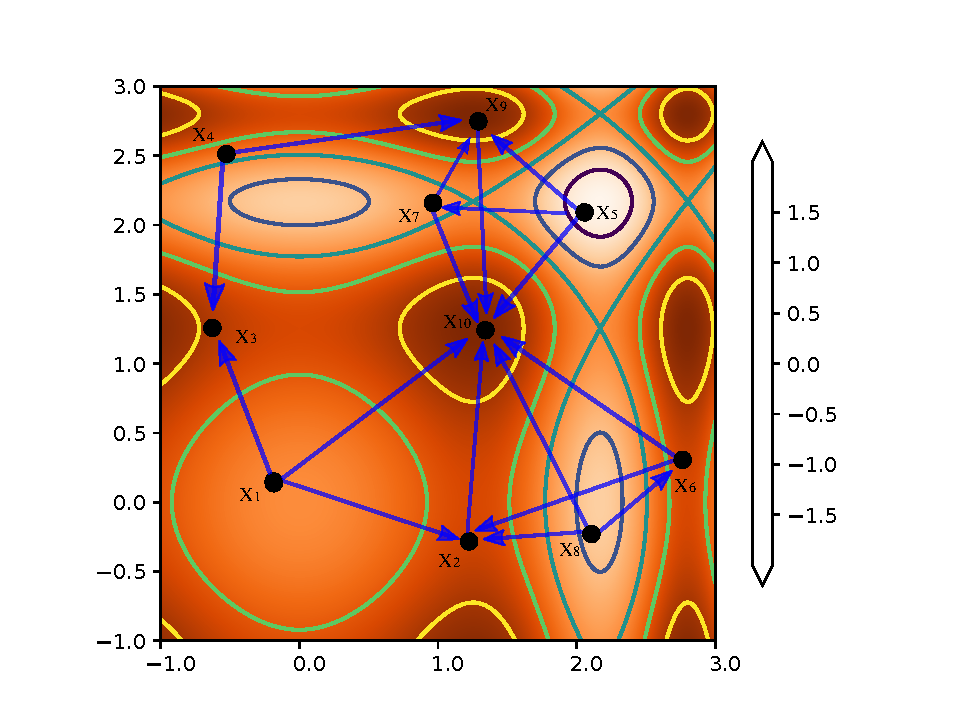
\includegraphics[scale=0.6]{fig_1.pdf}
\end{center}
\captionsetup{justification=centering}
\vspace*{-7mm} 
\caption{Contour plot of the function $f(x, y) = sen(x^2) + cos(y^2)$, and the graph based on the population.}\label{fig:Graph}
\end{figure*}


\subsection{Space Reduction}

In \cite{ITGO4} a heuristic for space reduction is proposed for the ITGO. After the individual selection step, a sub-space is created around every element, with space reduced in each dimension by $\phi \in (0, 1)$. A new population is generated for every space created, and new elements are selected, for each population. The process is repeated for a defined number of iterations until the execution of local search on selected elements of the last space reduction.

An example involving the application of this heuristic is presented in Fig. \ref{fig:SpaceReduction}, again for the function $f(x, y) = sen(x^2) + cos(y^2)$, in the domain $[-1, 3]^2$, with the first population composed by the same 10 points described previously. The Fig. \ref{fig:SpaceReduction-a} shows the selection of the points $\bm{x}_1$, $\bm{x}_5$ and $\bm{x}_8$, with a space reduced by $\phi = 0.25$. In the Fig. \ref{fig:SpaceReduction-b} we can observe the generation of populations for each new subspace. The red points are the individuals considered local optimum based on the topographic heuristic. It is worth noting that the local optimum points of the previous population are kept in the next population.


\begin{figure}[tp]
\centering
\begin{subfigure}{.5\textwidth}
  \centering
  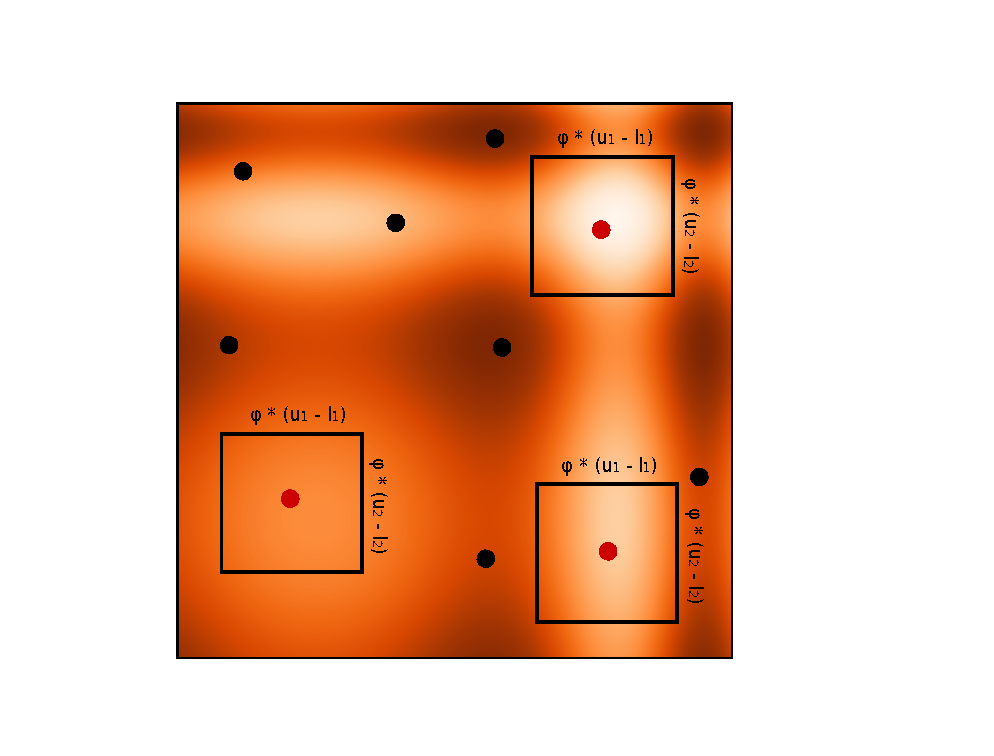
\includegraphics[width=1.1\linewidth]{fig_2.eps}
  \caption{}
  \label{fig:SpaceReduction-a}
\end{subfigure}%
\begin{subfigure}{.5\textwidth}
  \centering
  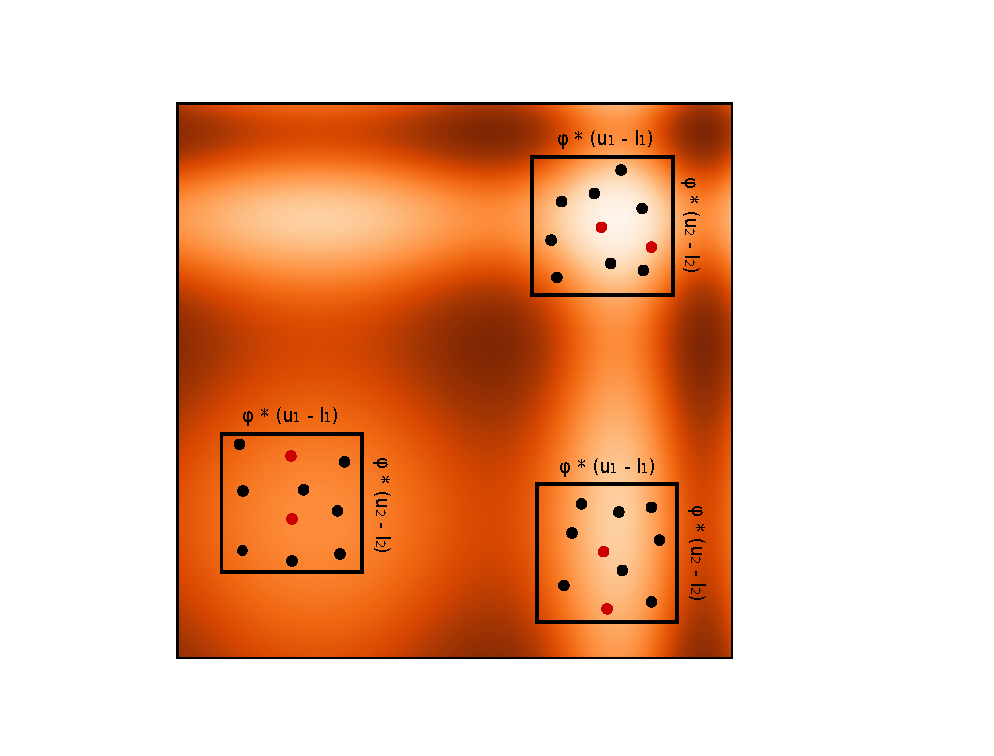
\includegraphics[width=1.1\linewidth]{fig_3.eps}
  \caption{}
  \label{fig:SpaceReduction-b}
\end{subfigure}
\caption{Example showing the application of the space reduction heuristic. In (a) we have the space reduction around the three individuals of Fig. 2 ($\bm{x}_1$, $\bm{x}_5$ and $\bm{x}_8$) in red (based on the topographical heuristic). In (b) are the respective populations generated in each restricted space to apply TGO.}\label{fig:SpaceReduction}
\end{figure}


At each iteration, a new population size is set, along with a new value for $K$, which is usually smaller than in the previous iteration.


\subsection{Constrained Optimization}

Until the moment, the ITGO algorithm was presented only for unconstrained optimization problems. ITGO was applied previously to constrained optimization problems \citep{ITGO2, ITGO3}, handling constraints by using a specific local search procedure or by penalizing infeasible individuals.

In this work, we propose a different approach, adopting a mechanism for comparing solutions proposed in \cite{ConHandling}, and used in some very competitive meta-heuristics, specially on differential evolution algorithms \citep{DE1, DE2, DE3}. As in this work is proposed a constrained version of ITGO, in the rest of this work, it is named as C-ITGO, standing for Constrained ITGO. The method for comparison comprises the three steps criteria:

\begin{itemize}

\item Between two feasible solutions, the fittest one is better.

\item A feasible solution is always preferred over an infeasible solution, irrespectively of its fitness.

\item Between two infeasible solutions, the one with the smallest sum of constraint violation (\ref{eq:viol}) is better.

\end{itemize}


In the topographical heuristic step, we compare two solutions using this three steps criteria with probability $\alpha$, and otherwise, we compare only the fitness value. What we try to achieve with this heuristic is keeping promising solutions with small violation of constraints for further exploration the local search step.

We generate a symmetric matrix of random numbers $R$, with $R_{i, j} = R_{j, i} \in [0, 1]$. If $R_{i, j} < \alpha$, then we compare elements $\bm{x}_i$ and $\bm{x}_j$ using the three steps criteria. Otherwise, only the fitness value is compared. In general, with this configuration, the number of local optimum points selected by the topographical heuristic is smaller, specially on problems with a small feasible area. 

An important thing to notice is that some distributions of the individuals, with populations of small size and a high value of $K$, may not generate any local optimum point in the topographical heuristic. In the case of none of the individuals are selected as local optimum given a population, we take the best individual according to the three step criteria as the only local optimum of that population. In practice, however, it is rather unusual to happen.

The best individual in the whole search is always selected using the three step criteria described above since  feasible solutions are generally preferred. In addition to this new topographical selection method, we also use local search algorithms for constrained optimization.


\subsection{Implementation}

We now present an overview of the implementation of the method, along with pseudocodes describing all necessary steps. Algorithm \ref{alg:ITGO} shows the general procedure for the C-ITGO algorithm.

The parameters are the functions $f(\cdot)$ and $v(\cdot)$, which return the function value and sum of constraints violation respectively, as defined in equations \ref{eq:func} and \ref{eq:viol}, the lower and upper bound vectors $\bm{l}$ and $\bm{u}$, the vector of population sizes $\bm{PS}$, the vector of the $K$ values $\bm{KS}$, the maximum number $Max\_LS$ of elements to execute the local search, the local search number of iterations $LS_1$ and $LS_2$, the space reduction factor $\phi$ and the probability for the three step comparison $\alpha$.



\begin{breakablealgorithm}
\caption{CI-TGO($f(\cdot)$, $v(\cdot)$, $\bm{l}$, $\bm{u}$, $\bm{PS}$, $\bm{KS}$, $Max\_LS$, $LS_1$, $LS_2$, $\phi$, $\alpha$)}
\label{alg:ITGO}
\begin{spacing}{1.5}
\begin{algorithmic}[1]

%\State $Population \gets \{\};$
\Statex
\State $\bm{best} \gets random(\bm{l}, \bm{u});$
%\NoNumber{}


\While{$Converged(\bm{best}) == \textbf{False}$}

\State $Populations \gets \{\bm{x} = \bm{x}^1, ..., \bm{x}^{\bm{PS}(1)} : \bm{x} \in random(\bm{l}, \bm{u}) \};$
\State $TopoBest \gets \{\};$

%\NoNumber{}

\For{$p \in \{1, ..., |\bm{PS}|\}$}
%\State $ps \gets \bm{PS}(numPs);$
\State $NewPops \gets \{\};$
%\NoNumber{}

\For{$pop \in Populations$}

\State $Topo_p \gets TopographicalHeuristic(f(\cdot), v(\cdot), pop, \bm{KS}(p), \alpha);$


\If{$p < |\bm{PS}|$}

\For{$\bm{x} \in Topo_p$}
\State $NewPops \gets NewPops \ \cup \ CreatePop(\bm{x}, \bm{l}, \bm{u},\bm{PS}(p+1), \phi^p);$
\EndFor

\Else
\State $TopoBest \gets TopoBest \cup Topo_p;$
\EndIf
\EndFor

\If{$p < |\bm{PS}|$}
\State $Populations \gets NewPops;$
\EndIf
\EndFor

\State $TopoBest \gets \{\bm{x} = \bm{x}^1, ..., \bm{x}^{min(|TopoBest|, Max\_LS)} : \bm{x} \in sort(TopoBest)\};$

\For{$\bm{x} \in TopoBest$}

\State $\bm{x} \gets LocalSearch(f(\cdot), v(\cdot), \bm{x}, LS_1);$


\If{$Compare(f(\cdot), v(\cdot), \bm{x}, \bm{best})$ \ \textbf{or} \ $f(\bm{x}) < f(\bm{best})$}

\State $\bm{x} \gets LocalSearch(f(\cdot), v(\cdot), \bm{x}, LS_2);$


\If{$Compare(f(\cdot), v(\cdot), \bm{x}, \bm{best})$}
\State $\bm{best} \gets \bm{x};$
\EndIf
\EndIf

\EndFor

\EndWhile

\State \Return $best;$


\end{algorithmic}
\end{spacing}
\algcomment{Pseudocode for Constrained I-TGO.}
\end{breakablealgorithm}


The first line initializes the vector $\bm{best}$ randomly within the range $[\bm{l}, \bm{u}]$, which is the variable that saves the best element found in the search. The main loop starts at line 2, where we check for convergence. The function $Converged$ is problem dependent and may take into account the number of iterations, the number of function calls, the convergence of the best individual or any other stopping criteria.

Line 3 initializes the vector of current populations, with $\bm{PS}(1)$ elements, with all elements inside the bounds of the problem $[\bm{l}, \bm{u}]$. The set $TopoBest$ at line 4 comprises the best local optimum elements found in all populations and is initialized empty. We use $rand$ here to denote the generation of a random scalar or vector for simplicity, although in the implementation we use Sobol sequences for the generation of the individuals.

For each population size (line 5), which is the number of space reductions plus one, we generate new populations, starting from the empty set at line 6. Here, we use $|\cdot|$ to denote the number of elements inside a set or a vector. Line 7 loops through all the populations and execute the topographical heuristic ($TopographicalHeuristic$ function), with $K = \bm{KS}(p)$. The variable $Topo_p$, at line 8, saves the local optimum points selected from the current population.

If the current space reduction is not the last ($p < |\bm{PS}|$, line 9), we create a new population around every point in the $Topo_p$ set, with size $\bm{PS}(p + 1)$ and space reduced at every dimension by $\phi^p$ (lines 10 and 11). Otherwise, if it is the last space reduction, we have to save the local optimum points in the set $TopoBest$ to apply local search (lines 12 and 13).\\[-1em]


\begin{breakablealgorithm}
\caption{CreatePop($\bm{x}$, $\bm{l}$, $\bm{u}$, $popSize$, $\phi$)}
\label{alg:CreatePop}
\begin{algorithmic}[1]

\State $\bm{l}' \gets max(\bm{l}, \bm{x} - (0.5 * \phi) * (\bm{u} - \bm{l}));$
\State $\bm{u}' \gets min(\bm{u}, \bm{x} + (0.5 * \phi) * (\bm{u} - \bm{l}));$
\State $Population \gets \{\bm{x} = \bm{x}^1, ..., \bm{x}^{popSize} : \bm{x} \in random(\bm{l}', \bm{u}')\};$

\State \Return $Population;$

\end{algorithmic}
\algcomment{Create a new population shrinked by $\phi$ around the point $\bm{x}$.}
\end{breakablealgorithm}


The $CreatePop$ procedure is shown in algorithm \ref{alg:CreatePop}. Given an individual $\bm{x}$ (a selected local optimum point), the function randomly generates a new population with $popSize$ individuals around that point, in the original space reduced by the fraction $\phi$. If the point is closer than $0.5 * (u_i - l_i), \ i = 1, ..., n$, from the lower or upper bounds at dimension $i$, the limits of that new population are taken to be the original bounds. The $min$ and $max$ operations are executed element by element.


At line 14, we check again, if the current space reduction is not the last, and update the current populations at line 15, if the condition holds. Line 16 selects the top $Max\_LS$ best elements of the set $TopoBest$, using the three steps criteria comparison as sorting criteria. If $|TopoBest| < Max\_LS$, we keep all the elements.

We loop through all the elements of the now sorted $TopoBest$ set at line 17, and apply local search, with at maximum $LS_1$ iterations, at line 18. The function $Compare$ (line 19) is the three step comparison, returning true if the first solution (third argument) is better than the second solution (fourth argument), and returns false otherwise. The element returned by the local search procedure is compared against the best element found in the whole search at line 19. If it is better than the best element found, or if its fitness is better, a new local search procedure is applied, now with $LS_2$ iterations, at line 20.

%The number of function calls is generally the determining factor of performance, so we wish to make the smallest number of local search iterations as possible since a call for the local search for each individual, in general, does hundreds or thousands of function evaluations.

The number of function calls is usually the determining factor of performance. So, we wish to do, as few local search iterations as possible, since a call to the local search for each individual typically makes hundreds or thousands of function evaluations. Here, we set $LS_2 > LS_1$, so every element undergoes $LS_1$ iterations of local search, but we only search finely for promising solutions, setting larger values for $LS_2$. Usually, the second local search is only necessary for problems where very finely tuned solutions are required.

At line 21 we compare again the solution generated by the second local search ($\bm{x}$) against the best found element ($\bm{best}$) using the three step criteria. If the new solution is better, we set $\bm{best}$ to that solution at line 22 and continue the loop for applying local search in the other elements. At the end of the execution, when $Converged$ in the outer loop returns true, we return the best solution found in the whole search at line 23. In practice, however, we 
may stop the algorithm as soon as the optimum solution is found or when the maximum number of function evaluations is exceeded.

The only thing left is the $TopographicalHeuristic$ procedure, shown in algorithm \ref{alg:TopographicalHeuristic}. The function takes as parameter the objective function $f(\cdot)$ and the sum of constraints function $v(\cdot)$, the current population to be evaluated, the value $K$ for the $KNN$ set, and the probability $\alpha$, for the three step comparison.


\begin{breakablealgorithm}
\caption{TopographicalHeuristic($f(\cdot)$, $v(\cdot)$, $Population$, $K$, $\alpha$)}
\label{alg:TopographicalHeuristic}
\begin{spacing}{1.5}
\begin{algorithmic}[1]


\State $M \gets |Population|;$
\State $\bm{best} \gets Population(0);$
\State $KNN_K \gets Build\_KNN(Population, K);$
\State $\bm{R} \gets random([0, 1]^{M \times M});$
\State $TopoBest \gets \{\};$
%\State $\bm{Dist}_{i, j} \gets \{|Population(i) - Population(j)|, \ i, j \in \{1, ..., |Population|\}\};$ 

\For{$i \in \{1, ..., |Population|\}$}

\State $insert \gets \bm{True};$

\For{$j \in \{1, ..., |Population|\} \ \cap \ \{\bm{x}_j \in KNN_K(\bm{x}_i)\}$}
	\If{$\bm{R}_{i, j} < \alpha$}
		\State $insert \gets insert$ \& $Compare(f(\cdot), v(\cdot), \bm{x}_i, \bm{x}_j);$
	\Else
		\State $insert \gets insert$ \& ($f(\bm{x}_i) < f(\bm{x}_j));$
	\EndIf
\EndFor

\If{$insert = \bm{True}$}
\State $TopoBest \gets TopoBest \ \cup \ \{\bm{x}_i\};$
\EndIf

\If{$Compare(f(\cdot), v(\cdot), \bm{x}_i, \bm{best})$}
\State $\bm{best} \gets \bm{x}_i;$
\EndIf
\EndFor

\If{$|TopoBest| = 0$}
	\State $TopoBest \gets \{\bm{best}\};$
\EndIf

\State \Return $TopoBest;$



\end{algorithmic}
\end{spacing}
\algcomment{Topographical heuristic procedure.}
\end{breakablealgorithm}


Lines 1-5 simply initialize the necessary structures. Namely, the number of elements $M$ in $Population$, the $\bm{best}$ vector, which is the best element of the entire population based on three step comparison (initially set to any individual of the population), the $\bm{KNN}_K$ structure based on the elements of the population, which is a mapping from a solution vector $\bm{x}$ to a set of the vectors that belong to the $\bm{KNN}_K$ of $\bm{x}$, the random symmetric matrix $R$, with every element in the range $[0, 1]$, and the $TopoBest$ set, containing the local optimum points, initially empty.

At line 6 we loop through all indices of $Population$, and set the $insert$ flag to $\bm{True}$ at line 7, which indicates if the individual $\bm{x}_i$ is a local optimum point. For every index $j$, such that $\bm{x}_j$ is in the set $\bm{KNN}_K(\bm{x}_i)$ (line 8), we compare $\bm{x}_j$ with $\bm{x}_i$. If $R_{i, j} < \alpha$, then we set the flag $insert$ to the boolean result of applying the \textit{and} operator ($\&$) to $insert$ and the result of $Compare$ (lines 9-10). That is, if $Compare$ returns false at least one time for any $j$, $insert$ will also be false for the index $i$. If $R_{i, j} >= \alpha$, then we make the same procedure, but now using fitness only comparison, at lines 11-12.

At line 13 we check if $insert = \bm{True}$, and, if so, $\bm{x}_i$ is a local optimum, and we insert it in the $TopoBest$ set, at line 14. Lines 15-16 selects the best element found in the whole population based on the three step comparison, and stores that solution in the variable $\bm{best}$. In case of no solution is selected as a local optimum, the set $TopoBest$ is composed only of the $\bm{best}$ element (lines 17-18). At line 19 we return the $TopoBest$ set, containing all the local optimum points (or the $\bm{best}$ element).


\subsection{Local Search}

In this section, we discuss the three different methods of local search used in C-ITGO and their implications on the final performance.

As we used Matlab to program C-ITGO, a natural choice for local search is the optimization toolbox. In the case of real non-linearly constrained problems, we used the \textit{SQP} (Sequential Quadratic Programming), present in the \textit{fmincon} package \citep{fmincon}. The basic SQP algorithm is described in Chapter 18 of \cite{Nocedal}, although the actual implementation used in fmincon uses some additional heuristics. 

A very successful method, also implemented in Matlab, that uses that same package (SQP of fmincon) is the \textit{MVMO} (Mean-Variance Mapping Optimization) \citep{MVMO}, winner of two different categories of the IEEE Congress on Evolutionary Computation competition on real optimization in 2016.

For mixed integer problems with nonlinear constraints, we used the \textit{OPTI} toolbox \citep{OPTI}, which have many algorithms specialized for mixed integer programming. Specifically, we used the \textit{BONMIN} (Basic Open-source Nonlinear Mixed INteger programming) \citep{BONMIN} and the \textit{NOMAD} (Nonlinear optimization with the MADS algorithm) \citep{NOMAD} solvers.

We emphasize here that any kind of local search can be used in conjunction with C-ITGO. We could use for example a specialized local search for a given problem. In this work, both problems on continuous and integer domains are treated in the same way, changing only the local search procedure.

It is true that some simpler problems can be solved solely by using an exact method such as those cited above, for example by calling the procedure at different random points. However, in multimodal objective functions with nonlinear constraints, it is usually infeasible. And even if a problem can be solved by an exact method, the number of function evaluations can be very large.

The objective is not to rely heavily on the local search procedure. Rather, what we want to achieve with the topographical heuristic is provide solutions close to a local or global optimum, so that any reasonably good local search can converge with relative ease. In this work, the maximum number of function evaluations allowed in the first call to the local search procedure is kept as small as possible, and, in most cases, it is enough to find optimal or nearly optimal solutions.



\subsection{Parameters}

Given the differences in the number of variables, constraints, size of the space, number of function calls taken by competing methods to converge and general complexity of the problems considered in this work, we selected experimentally specific parameters for each problem aiming to obtain the best performance of C-ITGO. This is a general approach taken for most of the optimization methods compared here. The parameters were selected so as to find optimal or near-optimal solutions while minimizing the number of function evaluations (NFEs).

Table \ref{tab:Parameters} shows the choice of the parameters for the eight engineering design problems we consider: Welded Beam (WB), Tension / Compression Spring (TC), Three-Bar truss (TB), Speed Reducer (SRI and SRII), Pressure Vessel (PV), Gear Train (GT) and Multiple Disk clutch brake (MD). We will comment each problem and the results obtained by C-ITGO and other competing methods in Section \ref{sec:Results}.


\begin{table*}[tp]
    \tiny
\begin{center}
\begin{tabular}{ | P{0.8cm} | P{0.8cm} | P{0.8cm} | P{0.8cm} | P{0.8cm} | P{0.8cm} | P{0.8cm} | P{0.8cm} | P{0.8cm} | P{0.9cm} | P{0.9cm}  | }
\hline
$\bm{Prob / \allowbreak Param}$ & $\bm{PS_1}$ & $\bm{PS_2}$ & $\bm{K_1}$ & $\bm{K_2}$ & $\bm{\alpha}$ & $\bm{\phi}$ & $\bm{LS1}$ & $\bm{LS2}$ & $\bm{MaxLS}$ & $\bm{LSType}$ \\
\hline

\textbf{WB} & 100 & 10 & 10 & 3 & 0.5 & 0.2 & 100 & 200 & 5 & \textbf{SQP} \\
\textbf{TC} & 50 & 10 & 8 & 3 & 0.5 & 0.2 & 100 & 200 & 5 & \textbf{SQP} \\
\textbf{TB} & 30 & 5 & 5 & 2 & 0.5 & 0.2 & 20 & 70 & 5 & \textbf{SQP} \\
\textbf{SRI} & 150 & 10 & 10 & 3 & 0.5 & 0.2 & 100 & 200 & 5 & \textbf{BONMIN} \\
\textbf{SRII} & 100 & 10 & 10 & 3 & 0.5 & 0.2 & 50 & 100 & 5 & \textbf{SQP} \\
\textbf{PV} & 50 & 10 & 8 & 3 & 0.5 & 0.5 & 30 & 100 & 5 & \textbf{BONMIN} \\
\textbf{GT} & 20 & 5 & 5 & 2 & 0.5 & 0.7 & 30 & 100 & 5 & \textbf{NOMAD} \\
\textbf{MD} & 20 & 5 & 7 & 2 & 0.5 & 0.7 & 100 & 200 & 5 & \textbf{NOMAD} \\
\hline

\end{tabular}
\end{center}
\vspace*{-6mm}
\caption{Parameters of C-ITGO for each engineering design problem. \\[1em]}
\label{tab:Parameters}
\end{table*}



For all problems, we only use a single space reduction, which generates two populations and two values for $K$, namely $PS_1$ (first population size, before space reduction) and $PS_2$ (second population size, after space reduction), and $K_1$ and $K_2$ (also before and after space reduction, respectively). The value for the probability $\alpha$ was kept constant for all problems, as well as the maximum number of elements to execute the local search, $MaxLs$. The value of $\phi$ was set to smaller values for problems defined on entirely continuous domains and assumed higher values for mixed integer problems. The $LS_1$ and $LS_2$ control the maximum number of allowed function evaluations in the local search in the first and second calls, respectively. Finally, $LSType$ represents the type of local search procedure used. %In next section, we discuss the three different methods of local search used and their implications on the final performance of the method.

The type of local search was determined based on the properties of each problem. For problems with only continuous variables, we used the SQP method (WB, TC, and TB). For problems with only discrete variables, we used the NOMAD solver (GT, MD), and for mixed integer problems, we used the BONMIN solver (SRI and PV). The only exception was SRII, in which we used the SQP algorithm rounding the variables that are required to be an integer. In tests with this specific problem, it resulted in better solutions than using the mixed integer solvers.


\section{Computational Results} \label{sec:Results}

The C-ITGO was implemented using Matlab, and the experiments were accomplished on a machine with the Intel i3-3110M CPU @2.40GHz processor with 4GB of RAM, running Windows 7. Also, we provide a free library for using C-ITGO for optimizing any user-defined function, being it constrained or not. The library uses by default the Matlab \textit{fmincon} solver for continuous problems and the OPTI toolbox (currently only readily available for Windows, but can be compiled for Linux and Mac as well) for mixed integer problems. Also, the user has the option to easily incorporate other local search algorithms, if desired.

%The source code for the reported results in this work can be found and downloaded for free at \cite{GIT}.

To evaluate the performance of the developed method to solve real-world problems, we use eight difficult constrained engineering optimization problems from the literature, whose objective functions and constraints are diverse (quadratic, cubic, polynomial and nonlinear) with many numbers and types of design variables (continuous, mixed and integer). 

In all tests, given the stochastic characteristic of C-ITGO, we run it 25 times, saving the Best and Worst feasible solutions, as well as the mean value (Mean) and standard deviation (SD) of the fitness after all runs. Given the great variability between the results found in the literature for most problems, we stop the execution of C-ITGO as soon as the best solution found in a run is considerably close to the optimum (the optimum solution for each of the eight engineering design problems considered is known). That is, the condition for stopping C-ITGO, when the fitness reaches a certain value, is problem dependent. At the end, the mean number of function evaluations (MNFEs) is reported for all runs.

Table \ref{tab:GAP} shows the values that determine the convergence of C-ITGO for each problem. The values in row \textit{GAP} represent the minimum Euclidean distance to the optimum that the fitness of a solution needs to be in order to stop the execution of C-ITGO. These values were chosen based on the results found by the competing methods, considering the variability of the precision of the reported solutions.

\begin{table*}[tp]
    \tiny
    \begin{center}
    
    \begin{tabular}{ P{1.2cm} P{1.2cm} P{1.2cm} P{1.2cm} P{1.2cm} P{1.2cm} P{1.2cm} P{1.2cm} P{1.2cm}  }
    \rule{0pt}{3ex}
    & \multicolumn{1}{|c}{WB} & TC & TB & SRI & SRII & PV & GT & MD  \\
    \hline
    \rule{0pt}{5ex}
    GAP & \multicolumn{1}{|c}{1E-6} & 1E-6 & 1E-5 & 1E-8 & 1E-7 & 1E-4 & 1E-10 & 1E-5 \\
    \end{tabular}
    \end{center}
    \vspace*{-3mm}
    \caption{Minimum distance to optimum to determine C-ITGO convergence for each problem. \\[1em]}
    \label{tab:GAP}
\end{table*}

The Gear Train (GT) was the only problem where we specified a maximum number of function evaluations. For this problem, if the NFEs reaches 800, we stop immediately and return the best solution found. It was necessary since the convergence requirements for this problem is very tight ($10E-10$). All other problems converged to at least \textit{GAP} of the optimum without the requirement to specify a maximum NFEs.

%The C-ITGO method finishes its execution when one or both of the two stop criteria is achieved: the convergence of the best individual or the maximum number of function calls is reached. Table \ref{tab:GAP} shows the values that determine the convergence of C-ITGO for each problem. The values in row GAP represent the minimum euclidean distance to the optimum that the fitness of a solution needs to be in order to stop the execution of C-ITGO. These values are chosen based on the results reported by the competing methods, considering the variability of the precision of the solutions among the problems.



In our tests, all solutions reported by C-ITGO are completely feasible for all problems. So, unless specified, we exclude from comparison methods that violate any constraint (unfeasible).

We compare 20 different optimization methods against C-ITGO. The most common meta-heuristic for solving the problems considered in this work is the Particle Swarm Optimization (PSO), including PSO-DE \citep{PSO-DE}, a hybrid PSO method combined with Differential Evolution (DE); the HPSO \citep{HPSO}, another hybridized particle swarm method in combination with simulated annealing; a co-evolutionary PSO denominated CPSO \citep{CPSO}; the hybridized PSO with Nelder-Mead simplex (NM-PSO) \citep{NM-PSO}; the Unified PSO (UPSO) \citep{UPSO}, a PSO variant that balances exploration and exploitation; the APSO, standing for Accelerated PSO  \citep{APSO}; the Gaussian Quantum-Behaved Particle Swarm Optimization methods, named QPSO and G-QPSO \citep{QPSO}; and the IPSO \citep{IPSO}, which incorporates an interval reducing procedure. More recently, and among the best PSO methods for constrained global optimization, we can cite the Improved Accelerated PSO algorithm (IAPSO) \citep{IAPSO}, which proposes some modifications and improves the APSO method.

Many other different optimization methods were also used for comparison in this work: the Mine Blast Algorithm (MBA) \citep{MBA}, a population-based optimization method based on the mine bomb explosion concept; the League Championship Algorithm (LCA) \citep{LCA}, which models a league championship environment with artificial teams; the Crossover-Based Artificial Bee Colony (CB-ABC) \citep{CB-ABC}, applying modified search operators over the regular ABC algorithm; the Differential Evolution with Level Comparison (DELC) \citep{DELC}, which converts a constrained problem into an unconstrained one by means of a level comparison mechanism; a Multi-View Differential Evolution (MVDE) \citep{MVDE}, which uses several different mutation strategies at every iteration; the Covariance Matrix Adaptation Evolution Strategy (CMA-ES) method \citep{CMA-ES}, which builds a distribution model of the population; the Water Cycle Algorithm (WCA) \citep{WCA}, a nature-inspired method based on the water cycle process; and the Cuckoo Search algorithm (CS) \citep{CS}, another nature-inspired method based on the cuckoo bird species behavior. Recently, reporting state-of-the-art results for some problems, we can cite the Improved Artificial Bee Colony with Modified Augmented Lagrangian (IABC-MAL) \citep{IABC-Mal}, which integrates the Modified Augmented Lagrangian method to handle constraints with the Improved ABC algorithm \citep{IABC}, and the Self-Adaptive Multi-Population based Jaya (SAMP-Jaya) algorithm \citep{SAMP-Jaya}, a multi-population scheme of the Jaya method \citep{Jaya}.


Following, the engineering optimization problems that will be tackled in this work will be briefly explained, as well as the solutions obtained by C-ITGO against the solutions of the best previously cited competing techniques of the literature. Further information on the Welded Beam (WB), Tension/Compression Spring (TC), Speed Reducer (SRI and SRII), Pressure Vessel (PV), Gear Train (GT) and Multiple Disk clutch brake (MD) problems can be found in the work of \cite{IAPSO}. The Three-Bar truss (TB) problem and additional information on Welded Beam (WB), Tension/Compression Spring (TC), Speed Reducer (SRI), Pressure Vessel (PV) and Gear Train (GT) can be seen in the work of \cite{MBA}.


We also decided to add in the appendix the initial results of applying the developed method to the GKLS class of problems \citep{GKLS}. We plan to improve C-ITGO further in a future work to better tackle unconstrained smooth optimization problems, comparing the results against a number of efficient deterministic global optimization methods.


\subsection{Welded beam design problem}


% !TEX root = ../ITGO.tex

\subsection*{Welded beam design problem}


The welded beam design \citep{WB} is the problem of minimizing the fabrication cost of a welded beam, subject to seven inequality constraints, being two linear and five nonlinear. The constraints include shear stress ($\tau$), bending stress in the beam ($\sigma$), buckling load on the bar ($Pc$), end deflection on the beam ($\delta$) and some more side constraints. The four design variables are continuous. The feasible best known objective value is $f(\bm{x}^*) = 1.7248523$. Figure \ref{fig:WB} presents the schematic of the welded beam design problem. \\


\begin{figure}[h]
    \begin{center}
    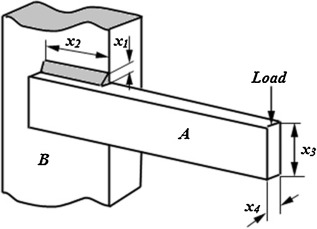
\includegraphics[scale=0.7]{Imgs/WB.jpg}
    \end{center}
    \captionsetup{justification=centering}
    \caption{Schematic view of the welded beam design problem.}\label{fig:WB}
\end{figure}


\prob{Appendix/Problems/WB}


We compare the results obtained by C-ITGO against a number of state-of-the-art methods used to solve this problem, including PSO-DE, HPSO, UPSO, MBA, CMA-ES, MVDE, CPSO, LCA, IPSO, CB-ABC, DELC, IABC-MAL, NM-PSO, APSO, WCA, IAPSO and SAMP-Jaya. Table \ref{tab:WB} shows the comparison of the statistical results obtained by all cited methods to solve the welded beam design problem. All the methods, with exception of CMA-ES, SAMP-Jaya and C-ITGO, took more than 10,000 iterations to achieve good quality solutions. C-ITGO achieved optimal solutions with a very small standard deviation of 3.65E-12, using ten times fewer function evaluations on average than most of the methods.

We write the statistics for the C-ITGO method in bold simply to highlight the reported results, not because it always presents the best statistics for all problems.


\begin{table*}[tp]
    \tiny
\begin{center}

\begin{tabular}{ P{2.0cm} P{2.0cm} P{2.0cm} P{2.0cm} P{2.0cm} P{2.0cm} P{2.0cm} P{2.0cm}  }
\hline
\textbf{Method} & \textbf{Best} & \textbf{Mean} & \textbf{Worst} & \textbf{SD} & \textbf{NFEs} \\
\hline
PSO-DE & 1.724852 & 1.724852 & 1.724852 & 6.70E-16 & 66,600 \\
HPSO & 1.724852 & 1.814295 & 1.749040 & 4.01E-02 & 81,000 \\
MBA & 1.724853 & 1.724853 & 1.724853 & 6.94E-19 & 47,340 \\
CPSO & 1.728024 & 1.748831 & 1.782143 & 1.29E-02 & 240,000 \\
LCA & 1.7248523 & 1.7248523 & 1.7248523 & 7.11E-15 & 15,000 \\
IABC-MAL & 1.724852 & 1.724852 & 1.724852 & 2.31E-12 & 15,000 \\
NM-PSO & 1.724717 & 1.726373 & 1.733393 & 3.50E-03 & 80,000 \\
IAPSO & 1.7248523 & 1.7248528 & 1.7248624 & 2.02E-06 & 12,500 \\
%Jaya & 1.724852 & 1.724852 & 1.724852 & 2.2E-08 & 4,739 \\
SAMP-Jaya & 1.724852 & 1.724852 & 1.724852 & 6.7E-16 & 3,618.25 \\
CI-TGO & 1.7248523 & 1.7248523 & 1.7248523 & 6.7E-16 & 1,166.84 \\


\hline
\end{tabular}
\end{center}

\caption{\fnt{8} Statistical results of different methods for Welded beam problem. \\[1em]}
\label{tab:WB}
\end{table*}



The results for C-ITGO and SAMP-Jaya are very similar, with the former having a slightly worse standard deviation, but converging in less than one-third of the number of function evaluations. We note here that the best solution achieved by NM-PSO is slightly unfeasible, so it should not be directly compared to the other methods.




\subsection{Tension/compression spring design problem}


% !TEX root = ../ITGO.tex

\subsection*{Tension/compression spring design problem}


This problem was introduced by \cite{TC}, and the objective is the minimization of the weight of a tension/compression spring (Figure \ref{fig:TC}). The problem has three continuous design variables, being them the diameter of spring wire ($x_1 = D$), the diameter of spring mean coil ($x_2 = d$) and the number of active coils ($x_3 = P$). It is subject to three nonlinear and one linear inequality constraints. The objective function value at the known global optimum is $f(\bm{x}^*) = 0.01266523$.

\begin{figure}[h]
\begin{center}
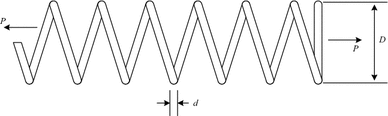
\includegraphics[scale=0.6]{Imgs/TC.png}
\end{center}
\captionsetup{justification=centering}
\caption{Schematic view of the tension/compression spring design problem.}\label{fig:TC}
\end{figure}


\prob{Appendix/Problems/TC}


A variety of methods were used in literature to solve the tension/compression spring design problem. Between them, we can cite CPSO, HPSO, NM-PSO, MBA, UPSO, PSO-DE, LCA, CB-ABC, QPSO, G-QPSO, APSO, CMA-ES, MVDE, DELC, WCA, IPSO, IAPSO, IABC-MAL and SAMP-Jaya. Table \ref{tab:TC} shows the statistical results of all methods, along with the number of function evaluations taken to achieve such results.


\begin{table*}[tp]
    \tiny
\begin{center}

\begin{tabular}{ P{2.0cm} P{2.0cm} P{2.0cm} P{2.0cm} P{2.0cm} P{2.0cm} P{2.0cm} P{2.0cm}  }
\hline
\textbf{Method} & \textbf{Best} & \textbf{Mean} & \textbf{Worst} & \textbf{SD} & \textbf{MNFEs} \\
\hline

HPSO & 0.012665 & 0.012719 & 0.012707 & 1.58E-05 & 81,000 \\
NM-PSO & 0.012630 & 0.012633 & 0.012631 & 8.47E-07 & 80,000 \\
MBA & 0.012665 & 0.012713 & 0.012900 & 6.30E-05 & 7,650 \\
PSO-DE & 0.012665 & 0.012665 & 0.012665 & 1.20E-08 & 24,950 \\
LCA & 0.01266523 & 0.01266541 & 0.01266667 & 3.88E-07 & 15,000 \\
CB-ABC & 0.012665 & 0.012671 & N/A & 1.42E-05 & 15,000 \\
QPSO & 0.012669 & 0.018127 & 0.013854 & 1.34E-03 & 2,000 \\
G-QPSO & 0.012665 & 0.017759 & 0.013524 & 1.27E-03 & 2,000 \\
APSO & 0.012700 & 0.013297 & 0.014937 & 6.85E-04 & 120,000 \\
CMA-ES & 0.01266524 & 0.01266861 & 0.01269335 & 6.30E-06 & 19,445 \\
MVDE & 0.01266527 & 0.01266732 & 0.01271906 & 2.45E-06 & 10,000 \\
DELC & 0.012665 & 0.012666 & 0.012665 & 1.30E-07 & 20,000 \\
IAPSO & 0.01266523 & 0.013676527 & 0.01782864 & 1.573E-3 & 2,000 \\
IABC-MAL & 0.01266523 & 0.01266525 & 0.01266539 & 6.78E-08 & 15,000 \\
SAMP-Jaya & 0.012664 & 0.013193 & 0.012714 & 9.25E-05 & 6,861 \\
C-ITGO & 0.01266523 & 0.01266523 & 0.01266525 & 2.81E-9 & 535.08 \\

\hline
\end{tabular}
\end{center}

\caption{\fnt{8} Statistical results of different methods for tension/compression spring design problem. \\[1em]}
\label{tab:TC}
\end{table*}




The methods vary greatly in the number of function evaluations required to converge to good quality solutions. Only three of the methods (QPSO, G-QPSO and IAPSO) achieved convergence with 2,000 function evaluations, while some methods required more than 100,000. The best solution achieved by all methods have the same fitness value up to five decimal places, with the exception of CPSO, UPSO, APSO and NM-PSO.
 
The best solution reported by NM-PSO is again unfeasible, so we do not compare it against other methods. The SAMP-Jaya method also seems to report a slightly unfeasible best solution, differing from the optimal value reported by other methods. However, the result achieved by SAMP-Jaya differs only at the sixth decimal place, and the difference may be due to wrong rounding. We cannot state this for sure since we do not have access to the solution vector found by the method. Given the differences between the precision in the solutions reported by the methods, we consider $f(\bm{x}) = 0.012665$ to be the fitness at the global optimum.

The C-ITGO method performed remarkably well on this problem, converging to the best solution found in 535.08 function evaluations on average, almost four times less than the second best competing method. Also, the standard deviation is very small, in the order of 2.81E-9. 

Given the relatively small domain of the problem, we believe that the C-ITGO method was able to cover the space efficiently, providing hot starting points for the local search method, which proved to be very effective in this case.




\subsection{Three-bar truss design problem}

% !TEX root = ../ITGO.tex

%\subsection*{Three-bar truss design problem}

The three-bar truss design problem \citep{TB} consists in minimizing the volume of a statically loaded three-bar truss. There are two continuous design variables and three nonlinear inequality constraints, based on the stress on each of the truss members ($\sigma$), with $f(\bm{x}^*) = 263.895843$. Figure \ref{fig:TB} shows the schematic view of the problem. The full problem statement follows:

\vspace{-0.5cm}

\input{Appendix/Problems/TB}

\vspace{0.5cm}


\begin{figure}[h]
    \begin{center}
    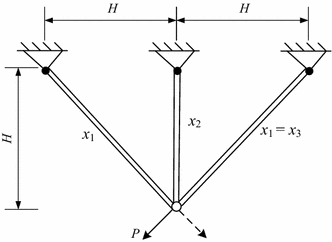
\includegraphics[scale=0.5]{Imgs/TB.png}
    \end{center}
    \captionsetup{justification=centering}
    \caption{Schematic view of the three-bar truss design problem.}\label{fig:TB}
\end{figure}



Here we present only the five best-performing methods used to solve this problem since the solutions found in the literature have very small variance from each other. These methods are PSO-DE, CMA-ES, MVDE, DELC, MBA and IABC-MAL. We present the statistical results for this problem in Table \ref{tab:TB}.


\begin{table*}[h]
    \tiny
\begin{center}

\begin{tabular}{ P{2.0cm} P{2.0cm} P{2.0cm} P{2.0cm} P{2.0cm} P{2.0cm} P{2.0cm} P{2.0cm}  }
\hline
\textbf{Method} & \textbf{Best} & \textbf{Mean} & \textbf{Worst} & \textbf{SD} & \textbf{MNFEs} \\
\hline

PSO-DE & 263.895843 & 263.895843 & 263.895843 & 4.50E-12 & 17,600 \\
CMA-ES & 263.895843 & 263.895843 & 263.895843 & 2.7E-09 & 1,706 \\
MVDE & 263.895843 & 263.895843 & 263.895855 & 2.58E-07 & 7,000 \\
DELC & 263.895843 & 263.895843 & 263.895843 & 4.3E-14 & 10,000 \\
MBA & 263.895852 & 263.897996 & 263.915983 & 3.93E-03 & 13,280 \\
IABC-MAL & 263.895843 & 263.895843 & 263.895843 & 0.0 & 15,000 \\
\textbf{C-ITGO} & \bf{263.895843} & \bf{263.895843} & \bf{263.895843} & \bf{2.0E-12} & \bf{136.48} \\


\hline
\end{tabular}
\end{center}
\vspace*{-6mm}
\caption{Statistical results of different methods for three-bar truss design problem. \\[1em]}
\label{tab:TB}
\end{table*}



From Table \ref{tab:TB} it is possible to note that all methods have very similar results, differing mainly in the number of function calls. This is not surprising, given that the problem is simpler, has fewer variables and consequently has a smaller domain than any other engineering design problem considered in this work.

C-ITGO achieved convergence quickly, taking 136.48 function evaluations on average. In this problem, we have set a small population, as well as a small number of function calls allowed in the local search procedure. Thus, we obtained the lowest MNFEs than any of the competing techniques, at least ten times lower. It seems that the solutions found by the topographical heuristic were already close to the optimum, so the local search converged in very few iterations. However, the C-ITGO method has a slightly worse standard deviation than DELC and IABC-MAL.



\subsection{Speed reducer design problem}

% !TEX root = ../ITGO.tex

%\subsection*{Speed reducer design problem}

In this problem, the total weight of the speed reducer (Figure \ref{fig:SR}) is to be minimized. The problem has seven design variables: face width ($b$), teeth module ($m$), number of teeth on the pinion ($z$), first and second length of shafts between bearings ($l_1$ and $l_2$) and first and second shafts diameter ($d_1$ and $d_2$) \citep{SR}. The problem has 11 nonlinear constraints, and the third variable is constrained to be an integer. A second version of the problem is also found in literature, where the only difference is in the lower bound of the fifth variable (7.8 for SR1 and 7.3 for SR2). The objective function value at the optimal is $f(\bm{x}^*) = 2996.34816497$ for the first version (SR1), and $f(\bm{x}^*) = 2994.471066$ for the second version (SR2). The mathematical formulation of the problem follows:

\vspace{-0.5cm}

\input{Appendix/Problems/SR1}

\vspace{0.5cm}

\begin{figure}[h]
    \begin{center}
    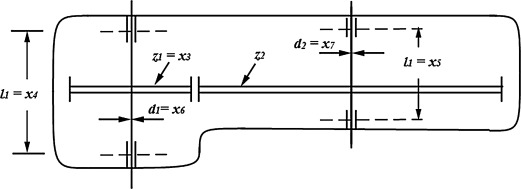
\includegraphics[scale=0.6]{Imgs/SR.jpg}
    \end{center}
    \captionsetup{justification=centering}
    \caption{Schematic view of the speed reducer design problem.}\label{fig:SR}
\end{figure}



For SRI, we compare C-ITGO results against four optimization methods, namely LCA, IPSO, APSO and IAPSO, shown in Table \ref{tab:SP1}.

The LCA, IPSO, IAPSO and C-ITGO present similar results, all finding the constrained global optimum solution and having very low standard deviation.



\begin{table*}[tp]
    \tiny
    \begin{center}
    
    \begin{tabular}{ P{2.0cm} P{2.0cm} P{2.0cm} P{2.0cm} P{2.0cm} P{2.0cm} P{2.0cm} P{2.0cm}  }
    \hline
    \textbf{Method} & \textbf{Best} & \textbf{Mean} & \textbf{Worst} & \textbf{SD} & \textbf{MNFEs} \\
    \hline
    
    SiC-PSO & 2996.34816 & 2996.4085 & NA & 0.0 & 24,000 \\
    COPSO & 2996.372448 & 2996.408525 & NA & 2.867E-02 & 30,000 \\
    LCA & 2996.34816497 & 2996.34816497 & 2996.34816497 & 2.63E-12 & 24,000 \\
    IPSO & 2996.34816497 & 2996.3481 & 2996.34816509 & 2.43E-18 & 20,000 \\
    IAPSO & 2996.34816497 & 2996.34816497 & 2996.34816497 & 6,88E-13 & 6,000 \\
    CI-TGO & 2996.34816497 & 2996.34816497 & 2996.34816497 & 7.5E-13 & 856.40 \\
        
    \hline
    \end{tabular}
    \end{center}
    
    \caption{\fnt{8} Statistical results of different methods for the speed reducer design problem I. \\[1em]}
    \label{tab:SP1}
    \end{table*}
    
    

The first three methods take at least 20,000 iterations to converge to good quality solutions, while IAPSO takes only 6,000 NFEs. C-ITGO outperforms the other methods by a large margin, converging in 858.40 function calls on average while maintaining negligible higher standard deviation than IAPSO and IPSO.

For this problem, we used considerably greater populations, of sizes 150 ($PS_1$) and 10 ($PS_2$), while maintaining the number of allowed function evaluations of the local search relatively small (100 and 200). For the worst case, C-ITGO took 3 full iterations to converge, while in most cases it converged in the first iteration.

For SRII, the methods used for comparison were PSO-DE, WCA, DELC, CB-ABC, CMA-ES, MVDE, IABC-MAL, LCA, APSO, MBA, IPSO, IAPSO and SAMP-Jaya. The reported results for the SAMP-Jaya method seems to violate the integer constraint at variable three, but it is included to show that even in harder situations the C-ITGO algorithm can still produce state-of-the-art results.

From Table \ref{tab:SP2}, we can see that DELC, CMA-ES, MVDE, IABC-MAL, LCA, IAPSO, SAMP-Jaya and C-ITGO are the only methods that converged to the optimum in every run, having very small standard deviation. Although similar results are observed regarding the quality of the solutions, C-ITGO converges much faster than any competing method, using seven times fewer function evaluations than SAMP-Jaya. The standard deviation achieved by C-ITGO is also only worse than the standard deviation reported by IABC-MAL (the difference is in the order of 1E-13), which took 15,000 function evaluations to converge.


\begin{table*}[h]
    \tiny
    \begin{center}
    
    \begin{tabular}{ P{2.0cm} P{2.0cm} P{2.0cm} P{2.0cm} P{2.0cm} P{2.0cm} P{2.0cm} P{2.0cm}  }
    \hline
    \textbf{Method} & \textbf{Best} & \textbf{Mean} & \textbf{Worst} & \textbf{SD} & \textbf{MNFEs} \\
    \hline
    
    PSO-DE & 2996.348167 & 2996.348174 & 2996.348204 & 6.40E-06 & 54,350 \\
    WCA & 2994.471066 & 2994.474392 & 2994.505578 & 7.4E-03 & 15,150 \\    
    DELC & 2994.471066 & 2994.471066 & 2994.471066 & 1.90E-12 & 30,000 \\
    CB-ABC & 2994.471066 & 2994.471066 & N/A & 2.48E-07 & 15,000 \\
    CMA-ES & 2994.471066 & 2994.471066 & 2994.471066 & 8.98E-10 & 12,998 \\
    MVDE & 2994.471066 & 2994.471066 & 2994.471066 & 2.82E-07 & 30,000 \\    
    IABC-MAL & 2994.471066 & 2994.471066 & 2994.471066 & 8.51E-13 & 15,000 \\ 
    LCA & 2994.471066 & 2994.471066 & 2994.471066 & 2.66E-12 & 24000 \\
    APSO & 3187.630486 & 3822.640624 & 4443.017639 & 366.146 & 30,000 \\
    MBA & 2994.482453 & 2996.769019 & 2999.652444 & 1.56 & 6300 \\
    IPSO & 2994.471067 & 2994.47108 & 2994.4711 & 9.27E-06 & 20,000 \\
    IAPSO & 2994.471066 & 2994.471066 & 2994.471066 & 2.65E-09 & 6,000 \\
    SAMP-Jaya & 2760.673988 & 2760.673988 & 2760.673988 & 2.54E-11 & 3744.66 \\    
    \textbf{C-ITGO} & \bf{2994.471066} & \bf{2994.471066} & \bf{2994.471066} & \bf{9.28E-13} & \bf{491.24} \\ 
    
  

    \hline
    \end{tabular}
    \end{center}
    \vspace*{-6mm}
    \caption{Statistical results of different methods for the speed reducer design problem II. \\[1em]}
    \label{tab:SP2}
    \end{table*}
    
    

For this specific problem, we used the SQP algorithm as local search and rounded the value of the third variable. In this case, this approach proved to converge much faster than using a mixed integer local search. Also, the first population size is considerably smaller than the one used in SRI (100 in this problem).



\subsection{Pressure vessel design problem}

% !TEX root = ../ITGO.tex

\subsection*{Pressure vessel design problem}

In the pressure vessel design problem, the objective is to minimize the total manufacturing cost, including the cost of the material, forming and welding costs \citep{PV}. The problem is subject to three linear and one nonlinear inequality constraint, and its structure is shown in Figure \ref{fig:PV}. The four variables are the thickness of the shell ($x_1 = T_s$), the thickness of the head ($x_2 = T_h$), the inner radius ($x_3 = R$), and the length of the cylindrical section of the vessel ($x_4 = L$). This is an example of a mixed integer problem, where the first and second variables are constrained to be integers. The value of the objective function at the best known feasible solution is around $f(\bm{x}^*) = 6059.7143$.

\begin{figure}[h]
    \begin{center}
    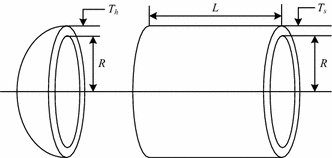
\includegraphics[scale=0.6]{Imgs/PV.png}
    \end{center}
    \captionsetup{justification=centering}
    \caption{Schematic view of pressure vessel design problem.}\label{fig:PV}
\end{figure}

\prob{Appendix/Problems/PV}


We compare C-ITGO against the UPSO, QPSO, G-QPSO, CMA-ES, MVDE, CB-ABC, PSO-DE, HPSO, WCA, LCA, APSO, CPSO, MBA, IPSO, DELC, IABC-MAL, SAMP-Jaya and IAPSO methods. The statistical results are shown in Table \ref{tab:PV}. Some of the methods used to solve this problem report unfeasible results (PSO-DE, WCA, MBA and SAMP-Jaya), probably either because the integer constraints are ignored or due to wrong rounding. Nevertheless, we still use the results of these methods to prove the superior convergence of C-ITGO, even in constrained mixed integer problems.



\begin{table*}[h]
    \tiny
    \begin{center}
    
    \begin{tabular}{ P{2.0cm} P{2.0cm} P{2.0cm} P{2.0cm} P{2.0cm} P{2.0cm} P{2.0cm} P{2.0cm}  }
    \hline
    \textbf{Method} & \textbf{Best} & \textbf{Mean} & \textbf{Worst} & \textbf{SD} & \textbf{MNFEs} \\
    \hline
    
    UPSO & 6544.2700 & 9032.5500 & N/A & 9.95E+02 & 100,000 \\
    QPSO & 6059.7209 & 8017.2816 & 6440.3786 & 4.79E+02 & 8,000 \\
    G-QPSO & 6059.7208 & 7544.4925 & 6440.3786 & 4.48E+02 & 8,000 \\
    CMA-ES & 6059.7143 & 6170.25055 & 6410.08676 & 140.4843 & 30,018 \\
    MVDE & 6059.7144 & 6059.99724 & 6090.53353 & 2.9103 & 15,000 \\ 
    CB-ABC & 6059.7143 & 6126.6237 & N/A & 1.14E+02 & 15,000 \\
    PSO-DE & 6059.7140 & 6059.7140 & N/A & N/A & 42,100 \\
    HPSO & 6059.7143 & 6099.9323 & 6288.6770 & 86.2000 & 81,000 \\
    WCA & 5885.3327 & 6198.6172 & 6590.2129 & 213.0490 & 27,500 \\
    LCA & 6059.8553 & 6070.5884 & 6090.6114 & 11.37534 & 24,000 \\
    APSO & 6059.7242 & 6470.7156 & 7544.4927 & 326.9688 & 200,000 \\
    CPSO & 6061.0777 & 6147.1332 & 6363.8041 & 86.4500 & 240,000 \\
    MBA & 5889.3216 & 6200.64765 & 6392.5062 & 160.34 & 70,650 \\    
    IPSO & 6059.7143 & 6059.7155 & 6059.7257 & 0.00232 & 20,000 \\
    DELC & 6059.7143 & 6059.7143 & 6059.7143 & 2.10E-11 & 30,000 \\  
    IABC-MAL & 6059.7143 & 6072.5972 & 6089.2720 & 1.88E-06 & 15,000 \\
    SAMP-Jaya & 5872.2129 & 5872.2129 & 5872.2129 & 5.0E-12 & 6513.33 \\    
    IAPSO & 6059.7143 & 6068.7539 & 6090.5314 & 14.0057 & 7,500 \\
    \textbf{C-ITGO} & \bf{6059.7143} & \bf{6059.7143} & \bf{6059.7143} & \bf{9.8E-13} & \bf{1101.64} \\
    
    \hline
    \end{tabular}
    \end{center}
    \vspace*{-6mm}
    \caption{Statistical results of different methods for the pressure vessel design problem. \\[1em]}
    \label{tab:PV}
    \end{table*}
    
    


The algorithms CMA-ES, CB-ABC, HPSO, IABC-MAl, IPSO, DELC, IAPSO and C-ITGO are the only who found the feasible optimal solution. All other methods presented relatively poor performance, with much higher NFEs on average. C-ITGO takes less than five times the number of function evaluations to converge than the best competing method, SAMP-Jaya, which reported a result of 6513.33 MNFEs. Also, C-ITGO achieves the smallest standard deviation among all methods. All runs of C-ITGO converged quickly to the known global optimum, showing unarguably better results than any other method compared in this problem.



\subsection{Gear train design problem}

% !TEX root = ../ITGO.tex

In this problem, the objective is to minimize the cost of the gear ratio of the gear train \citep{PV}. An example is shown in Figure \ref{fig:GT}. The problem has four variables, representing the number of teeth for the four gears ($x_1 = A$, $x_2 = B$, $x_3 = D$, and $x_4 = F$), with $f(\bm{x}^*) = 2.700857E \! - \! 12$. The only constraint of the problem is that all variables must be integers. The full problem statement follows:

\vspace{-0.5cm}

\input{Appendix/Problems/GT}

\vspace{0.5cm}


\begin{figure}[h]
    \begin{center}
    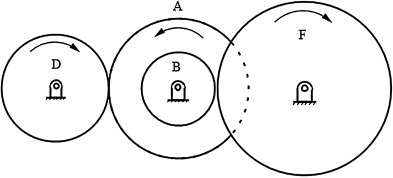
\includegraphics[scale=0.6]{Imgs/GT.jpg}
    \end{center}
    \captionsetup{justification=centering}
    \caption{Gear train design problem structure.}\label{fig:GT}
\end{figure}



We compare the C-ITGO results, shown in Table \ref{fig:GT}, against other five methods: MBA, UPSO, CS, APSO and IAPSO. In general, all methods compared achieved similar results, having found the global optimal solution for the problem. The main difference relies on the number of function calls, varying from 100,000 for UPSO to 800 for IAPSO.


\begin{table*}[tp]
    \tiny
\begin{center}

\begin{tabular}{ P{2.0cm} P{2.0cm} P{2.0cm} P{2.0cm} P{2.0cm} P{2.0cm} P{2.0cm} P{2.0cm}  }
\hline
\textbf{Method} & \textbf{Best} & \textbf{Mean} & \textbf{Worst} & \textbf{SD} & \textbf{MNFEs} \\
\hline

MBA & 2.700857E-12 & 2.062904E-08 & 2.47E-09 & 3.94E-09 & 1120 \\
UPSO & 2.700857E-12 & 3.80562E-08 & N/A & 1.09E-07 & 100,000 \\
CS & 2.7009E-12 & 1.9841E-9 & 2.3576E-9 & 3.55E-9 & 5,000 \\
APSO & 2.700857E-12 & 4.781676E-07 & 7.072678E-06 & 1.44E-06 & 8,000 \\
IAPSO & 2.700857E-12 & 5.492477E-09 & 1.827380E-08 & 6.36E-09 & 800 \\
C-ITGO & 2.700857E-12 & 4.6504232E-09 & 2.7264505E-08 & 6.85E-09 & 773.0 \\


\hline
\end{tabular}
\end{center}
\vspace*{-6mm}
\caption{Statistical results of different methods for the gear train design problem. \\[1em]}
\label{tab:GT}
\end{table*}




Since this is an integer optimization problem, we used the mixed integer local search based on the NOMAD solver. In this problem, the solver had some difficulty in some runs, achieving 6.85E-09 of standard deviation, more than IAPSO, CS and MBA. The mean fitness value, however, is just worse than the CS method, which takes 5,000 function calls to converge. Besides this drawbacks, C-ITGO was the fastest method to achieve convergence, taking only 773.0 function calls on average.



\subsection{Multiple disk clutch brake design problem}

% !TEX root = ../ITGO.tex

%\subsection*{Multiple disk clutch brake design problem}

This is also an example of a problem where all variables are discrete. The Multiple disk clutch brake design problem aims at minimizing the mass of a multiple disk clutch brake \cite{MD}. There are five integer variables: the inner radius ($x_1$), outer radius ($x_2$), thickness of the disk ($x_3$), actuating force ($x_4$) and number of friction surfaces ($x_5$) (Figure \ref{fig:MD}). The problem is also constrained by nine nonlinear inequalities. The objective function at the optimal solution is $f(\bm{x}^*) = 0.313656$. The mathematical formulation of the problem follows:

\vspace{-0.5cm}

\input{Appendix/Problems/MD}

\vspace{0.5cm}


\begin{figure}[h]
    \begin{center}
    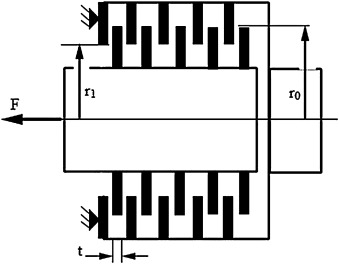
\includegraphics[scale=0.6]{Imgs/MD.jpg}
    \end{center}
    \captionsetup{justification=centering}
    \caption{Schematic view of the multiple disk clutch brake design problem.}\label{fig:MD}
\end{figure}


To compare the results, we used only methods who achieved close performance to the obtained by C-ITGO, since some methods in literature have very diverging results. The methods compared are WCA, IPSO, APSO and IAPSO. The WCA, IPSO, and IAPSO methods achieved good performance in this problem, finding the global optimal solution and having very small variance, as shown in Table \ref{tab:MD}. The WCA and IAPSO took very few function evaluations to converge, respectively 500 and 400. IPSO took long more, with 20,000 function evaluations. However, the reported standard deviation for IPSO was 0.0.


\begin{table*}[tp]
    \tiny
    \begin{center}
    
    \begin{tabular}{ P{2.0cm} P{2.0cm} P{2.0cm} P{2.0cm} P{2.0cm} P{2.0cm} P{2.0cm} P{2.0cm}  }
    \hline
    \textbf{Method} & \textbf{Best} & \textbf{Mean} & \textbf{Worst} & \textbf{SD} & \textbf{NFEs} \\
    \hline

    WCA & 0.313656 & 0.313656 & 0.313656 & 1.69E-16 & 500 \\
    IPSO & 0.313656 & 0.313656 & 0.313656 & 0.0 & 20,000 \\
    IAPSO & 0.313656 & 0.313656 & 0.313656 & 1.13E-16 & 400 \\
    CI-TGO & 0.313656 & 0.313656 & 0.313656 & 1.13E-16 & 286.48 \\

    \hline
    \end{tabular}
    \end{center}
    
    \caption{\fnt{8} Statistical results of different methods for the multiple disk clutch break design problem. \\[1em]}
    \label{tab:MD}
    \end{table*}
    
    

The C-ITGO clearly outperforms the other methods, having a standard deviation of 1.13E-16, while converging with only 286.48 function evaluations on average. For this problem, we used very small populations, of sizes 20 ($PS_1$) and 5 ($PS_2$). The number of function evaluations in the first step was 100, and most runs converged in much less, enjoying the quality of initial solutions provided by the topographical heuristic step. Some runs, however, took more than 1,000 function evaluations, bringing the mean NFEs up.



\subsection{Best Solutions to the Engineering Problems}

Table \ref{tab:BestResults} shows the fitness value, the values of the variables and the values of the constraints for the best solution found by C-ITGO for all problems. The precision of the results of each problem was set to match the results reported by the competing methods cited in this work. However, to the best of our knowledge, the best solution found by C-ITGO for each problem is equal to, or negligibly worse (up to several decimal places) than the best solutions reported by state-of-the-art methods.


\noindent
\begin{table*}[tp]
    \tiny
\begin{center}
\begin{adjustwidth}{-1cm}{}
\begin{tabular}{ | P{1.0cm} | P{1.5cm} |  P{1.5cm} | P{1.5cm} | P{1.5cm} | P{1.5cm} | P{1.5cm} | P{1.5cm} | P{1.5cm} |  }
\hline
\textbf{Prob.} & \textbf{WB} & \textbf{TC} & \textbf{TB} & \textbf{SRI} & \textbf{SRII} & \textbf{PV} & \textbf{GT} & \textbf{MD} \\
\hline
\rule{0pt}{3ex}
$f(\cdot)$ & 1.7248523 & 0.01266523 & 263.895843 & 2996.34816497 & 2994.471066 & 6059.7143 & 2.700857E-12 & 0.313656 \\
\hline
\rule{0pt}{3ex}
$\bm{x}_1$ &  0.2057296 & 0.05168906 & 0.788675 & 3.5 & 3.5 & 13.0 & 43 & 70  \\
$\bm{x}_2$ &  3.4704886 & 0.35671774 & 0.408248 & 7.0 & 0.7 & 7.0 & 16 & 90 \\
$\bm{x}_3$ &  9.0366239 & 11.28896574 & & 17 & 17 & 41.5984 & 19 &  1  \\
$\bm{x}_4$ &  0.2057296 & & & 7.3 & 7.3 & 176.6366 & 49 & 830  \\
$\bm{x}_5$ & & & & 7.8 & 7.715320 & & & 3 \\
$\bm{x}_6$ & & & & 3.35021467 & 3.350215 & & &   \\
$\bm{x}_7$ & & & & 5.28668323 & 5.286654 & & &   \\
\hline
\rule{0pt}{3ex}
$\bm{g}_1$ & 0.0 & 0.0 & 0.0 & -0.07391528 & -0.073915 & -2.6645E-15 & & 0.0  \\
$\bm{g}_2$ & 0.0 & 0.0 & -1.464102 & -0.19799853 & -0.197999 & -0.0359 & & -24.0  \\
$\bm{g}_3$ & 0.0 & -4.05378563 & -0.535898 & -0.49917225 & -0.499172 & -4.4238E-09 & & -0.917438 \\
$\bm{g}_4$ & -3.4329838 & -1.09159320 & & -0.90147170 & -0.904644 & -63.3634 & & -9.826183  \\
$\bm{g}_5$ & -0.0807296 & & & -8.846257E-13 & -2.220446E-16 & & &  -7.894697 \\
$\bm{g}_6$ & -0.2355403 & & & -4.885758E-12 & 0.0 & & & -0.173855  \\
$\bm{g}_7$ & -1.818989E-12 & & & -0.7025 & -0.7025 & & & -40.118750 \\
$\bm{g}_8$ & & & & -1.887379E-15 & 0.0 & & &  -14.826145 \\
$\bm{g}_9$ & & & & -0.58333333 & -0.583333 & & &    \\
$\bm{g}_{10}$ & & & & -0.05132575 & -0.051326 & & &    \\
$\bm{g}_{11}$ & & & & -0.01085237 & 0.0 & & &    \\
\hline
\end{tabular}
\end{adjustwidth}
\end{center}
\vspace*{-6mm}
\caption{Results for the best solution found by C-ITGO for each engineering design problem.. \\[1em]}
\label{tab:BestResults}
\end{table*}




\subsection{Statistical Tests To Analyse the Computational Results}

We now prove the significant improvement of C-ITGO over the competing methods by means of a nonparametric statistical test, where no assumptions are made regarding the underlying distribution of the data. Since no other algorithm than C-ITGO solves all the eight engineering design problems presented in this paper, we cannot apply typical statistical methods, such as the Friedman test \citep{Friedman}.

Instead, we use the Skillings-Mack test \citep{Skillings}, which is a Friedman\allowbreak-type statistical test that can be used when there are missing data, and that reduces to the Friedman test when the data has no missing entries. Just as in the Friedman test, the Skillings-Mack test finds the rank of the competing algorithms for each problem and then calculates the mean or average rank. The lower the mean rank, the better is the performance of the algorithm. The Skillings-Mack statistical test is also useful when there are many ties or equal ranks, as well as for small samples.

The method reports a \textit{p-value}, the probability that, when the null hypothesis is assumed to be true (in this case, no difference between the performance of the optimization methods), the results observed by the experiments at hand are at least of the same magnitude that the true values that would be observed in the limit of an infinite number of samples. Thus, a small p-value, say less than 0.05, represents a high chance that the null hypothesis is false.

In this work, the mean number of function evaluations (MNFEs) is used as the comparing metric. We used the \textit{Skillings.Mack} package \citep{SkillMack} of the \textit{R} language \citep{R} to report the following results.

In Table \ref{tab:SkillMack_3} we show the results of applying the statistical test to all the methods that solved at least three of the eight engineering design problems considered in this work. The mean rank of C-ITGO is 1.0, given that it has the smallest MNFEs for all problems. That is much less than IAPSO and SAMP-Jaya, which have a mean rank of 2.75. The mean ranks are also shown in the form of a bar plot for all methods in Figure \ref{fig:SkillMack_3}.


\begin{table}[h]
    \tiny
    \begin{center}
    
    \begin{tabular}{ P{2.0cm} P{2.0cm} P{2.0cm} P{2.0cm} P{2.0cm} P{2.0cm}  }
    \rule{0pt}{3ex}
    \textbf{p-value} & \bf{7E-06} & \multicolumn{3}{c}{}  \\
    \cline{1-2}
    \rule{0pt}{5ex}

    & & \multicolumn{2}{c}{\textbf{Methods}} & & \\
    \rule{0pt}{5ex}

    & C-ITGO & IAPSO & SAMP-Jaya & IABC-Mal & PSO-DE \\
    \textbf{Mean rank} & 1.0 & 2.6875 & 3.0625 & 5.0 & 6.6875 \\
    \hline
    
    \rule{0pt}{7ex}

    & HPSO & MBA & LCA & CB-ABC & DELC \\
    \textbf{Mean rank} & 6.8125 & 5.125 & 5.375 & 4.5625 & 5.8125 \\
    \hline

    \rule{0pt}{7ex}
    
    & CMA-ES & MVDE & IPSO & WCA & APSO \\
    \textbf{Mean rank} & 4.5625 & 4.8125 & 5.375 & 5.25 & 7.9375 \\
    
    \hline
    \end{tabular}
    \end{center}
    \vspace*{-4mm}
    \caption{Skillings-Mack test for methods solving at least three problems. \\[1em]}
    \label{tab:SkillMack_3}
\end{table}


As shown in Table \ref{tab:SkillMack_3}, the value of the Skillings-Mack statistic is 63.66813949 with an approximate p-value of 1.2469E-07 calculated from the chi-squared distribution with 16 degrees of freedom, which strongly implies that the null hypothesis does not hold true at the critical level of $\alpha$ = 0.05 or $\alpha$ = 0.01. That is, there is at least one method that is significantly better than the others. 



\begin{figure}[h]
    \begin{center}
    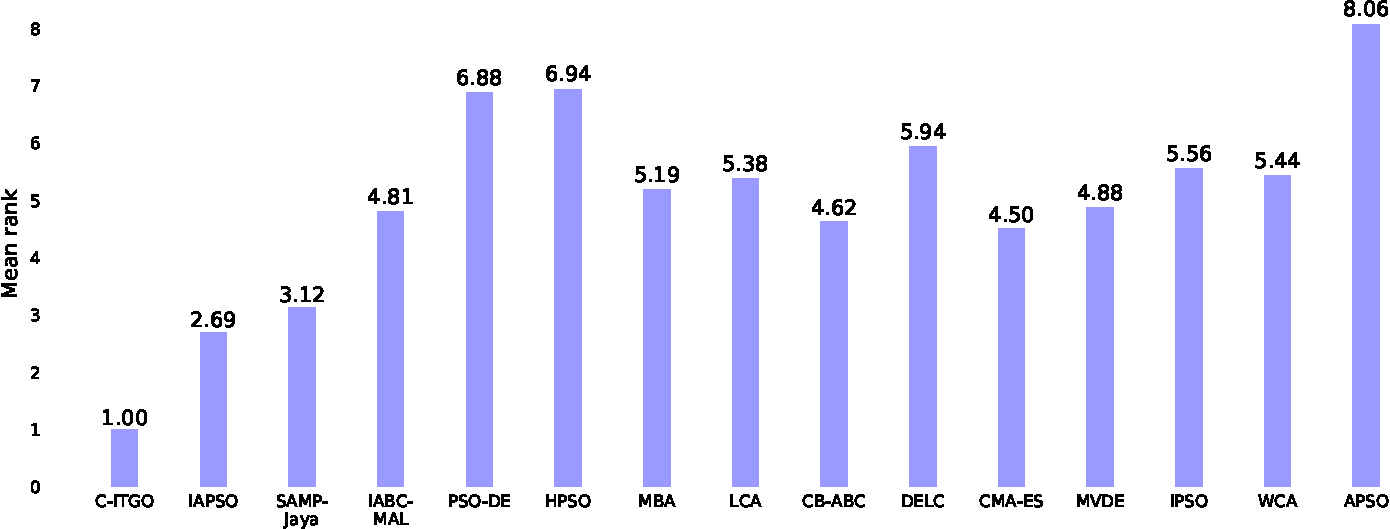
\includegraphics[scale=0.6]{Imgs/SkillMack_3-crop.pdf}
    \end{center}
    \captionsetup{justification=centering}
    \vspace*{-4mm}
    \caption{Mean rank plot for all methods that solve at least three problems.}\label{fig:SkillMack_3}
\end{figure}



We also show in Table \ref{tab:SkillMack_5} the results of applying the Skillings-Mack test to the methods that solved at least five problems. For this case, the value of the Skillings-Mack statistic is 44.23462786 with an approximate p-value of 7E-06 calculated from the chi-squared distribution with 11 degrees of freedom. The difference between the results reported in Table \ref{tab:SkillMack_3} is mainly due to the reduction of the number of methods, and the exclusion of some methods that performed well, but in four or fewer problems, such as SAMP-Jaya.

\begin{table}[h]
    \tiny
    \begin{center}
    
    \begin{tabular}{ P{2.0cm} P{2.0cm} P{2.0cm} P{2.0cm} P{2.0cm}  }
    \rule{0pt}{3ex}
    \textbf{p-value} & \bf{8.3E-05} & \multicolumn{3}{c}{}  \\
    \cline{1-2}
    \rule{0pt}{5ex}

    & \multicolumn{2}{c}{\textbf{Methods}} & \\
    \rule{0pt}{5ex}

    & C-ITGO & IAPSO & IABC-MAL & MBA \\
    \textbf{Mean rank} & 1.0 & 2.25 & 3.8125 & 4.0 \\
    \hline
    
    \rule{0pt}{7ex}

    & LCA & CMA-ES & MVDE & APSO \\
    \textbf{Mean rank} & 4.0 & 3.5625 & 3.6875 & 5.6875 \\
    \hline


    \hline
    \end{tabular}
    \end{center}
    \vspace*{-4mm}
    \caption{Skillings-Mack test for methods solving at least five problems. \\[1em]}
    \label{tab:SkillMack_5}
\end{table}

\begin{figure}[bp]
    \begin{center}
    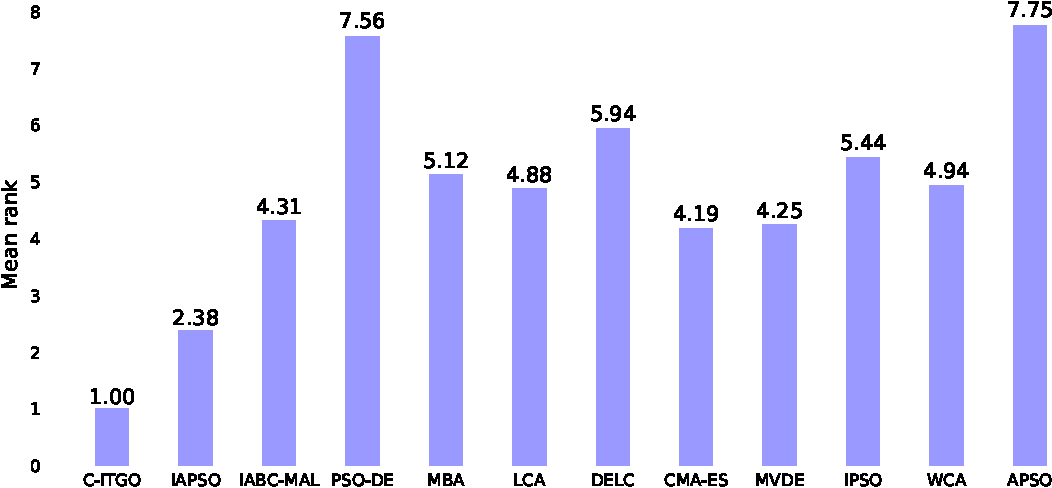
\includegraphics[scale=0.6]{Imgs/SkillMack_5-crop.pdf}
    \end{center}
    \captionsetup{justification=centering}
    \vspace*{-4mm}
    \caption{Mean rank plot for all methods that solve at least five problems.}\label{fig:SkillMack_5}
\end{figure}

We see again that C-ITGO has a mean rank of 1.0, far less than IAPSO with 2.375, standing in second place. The plot for the mean rank is shown in Figure \ref{fig:SkillMack_5}. The p-value (7E-06) for this case is also very small, rejecting the null hypothesis at critical level of $\alpha$ = 0.05 or $\alpha$ = 0.01.


We also present in Table \ref{tab:SignedTest} the results of applying the pairwise signed test, comparing C-ITGO against the same methods presented in Table \ref{tab:SkillMack_5} and considering the same performance metric. Here, a "+" represents that C-ITGO outperforms the corresponding method, a "=" represents a tie, and a "-" represents a loss (C-ITGO has worse performance than the corresponding method). If a method does not solve a certain problem, that entry is ignored (marked with "*"). The last row shows the final sum of the number of "+", "=" and "-" for all methods.

\begin{table}[h]
    \tiny
    \begin{center}

    \begin{tabular}{ P{0.7cm} P{0.7cm} P{0.7cm} P{0.8cm} P{0.7cm} P{0.7cm} P{0.7cm} P{0.7cm} P{0.7cm} P{0.7cm} P{0.7cm} P{0.7cm} P{0.7cm}  }
    

    \textbf{Eng. Prob.} & \multicolumn{1}{|c}{C-ITGO} & IAPSO & IABC-MAL & PSO-DE & MBA & LCA & DELC & CMA-ES & MVDE & IPSO & WCA & APSO  \\
    \hline


    \rule{0pt}{5ex}
    WB & \multicolumn{1}{|c}{\textbf{940.68}}     & 12,500 & 15,000 & 66,000 & 47,340 & 15,000 & 20,000 & 4,658 & 15,000 & 20,000 & 46,450 & 50,000 \\
       &                  \multicolumn{1}{|c}{}   &    +   &    +   &    +   &    +   &    +   &    +  &    +   &  +     &    +   &   +    &    +   \\

    \rule{0pt}{7ex}
    TC & \multicolumn{1}{|c}{\textbf{535.08}} & 2,000 & 15,000 & 24,950 & 7,650 & 15,000 & 20,000 & 19,445 & 10,000 & 20,000 & 11,750 & 120,000 \\
       &   \multicolumn{1}{|c}{}              &    +  &    +   &    +  &    +   &    +   &    +   &   +    &    +   &     +  &    +   &    +    \\

    \rule{0pt}{7ex}
    TB & \multicolumn{1}{|c}{\textbf{136.48}} & * & 15,000 & 17,600 & 13,280 & * & 10,000 &  1,706 & 7,000 & * & * & * \\
       &           \multicolumn{1}{|c}{}      &   &    +   &    +   &    +   &   &   +    &   +   &    +   &   &   &  \\

    \rule{0pt}{7ex}
    SRI & \multicolumn{1}{|c}{\textbf{856.40}} & 6,000 & * & * & * & 24,000 & * & * & * & 20,000 & * & 30,000 \\
        &           \multicolumn{1}{|c}{}      &    +  &   &   &   &    +   &   &   &   &    +   &   &    +   \\

    \rule{0pt}{7ex}
    SRII & \multicolumn{1}{|c}{\textbf{491.24}} & 6,000 & 15,000 & 54,350 & 6,300 & 24,000 & 30,000 & 12,998 & 30,000 & 20,000 & 15,150 & 30,000 \\
         &  \multicolumn{1}{|c}{}               &    +  &    +   &   +    &    +  &    +   &    +   &    +   &    +   &   +    &   +    &    +    \\


    \rule{0pt}{7ex}
    PV  & \multicolumn{1}{|c}{\textbf{1101.64}} & 7,500 & 15,000 & 42,100 & 70,650 & 24,000 & 30,000 & 30,018 & 15,000 & 20,000 & 27,500 & 200,000 \\
        &   \multicolumn{1}{|c}{}               &    +  &    +   &   +    &   +    &    +   &   +    &    +   &    +   &    +   &   +    &   +     \\

    \rule{0pt}{7ex}
    GT  & \multicolumn{1}{|c}{\textbf{773.0}} & 800 & * & * & 1,120 & * & * & * & * & * & * & 8,000 \\
        &   \multicolumn{1}{|c}{}             &  +  &   &   &   +  &   &   &   &    &   &   &  +   \\


    \rule{0pt}{7ex}
    MD  & \multicolumn{1}{|c}{\textbf{286.48}} & 400 & * & * & * & * & * & * & * & 20,000 & 500 & 2,000 \\
        &   \multicolumn{1}{|c}{}              &  +  &   &   &  &   &   &   &  &   +    &  +  &  +   \\

    \hline
    
    \rule{0pt}{5ex}
     \textbf{+/=/-} &  \multicolumn{1}{|c}{}  &   \textbf{7/0/0} &   \textbf{5/0/0} &  \textbf{5/0/0} &  \textbf{6/0/0} &  \textbf{5/0/0} &  \textbf{5/0/0} &  \textbf{5/0/0} &  \textbf{5/0/0} &   \textbf{6/0/0} &   \textbf{5/0/0} &   \textbf{7/0/0}  \\
        



    \end{tabular}
    \end{center}
    \captionsetup{justification=centering}
    \caption{The signed test comparing C-ITGO against the other methods that solved at least five problems. Empty entries are represented by *. \\[1em]}
    \label{tab:SignedTest}
\end{table}

As we can see from Table \ref{tab:SignedTest}, C-ITGO always has a better MNFEs than any method for all problems, so there are only "+" entries. Following the guidelines presented in \cite{Friedman}, we can conclude that C-ITGO always achieves a p-value of at least 0.05 when compared to the methods of Table \ref{tab:SignedTest}.


To prove the superior convergence of C-ITGO, we present one more nonparametric statistical test, the Wilcoxon signed rank test, also described in \cite{Friedman}. This is a more robust approach to a pairwise statistical comparison than the previous test, that aims to detect a significant difference between the means of two competing techniques. 

The results shown in Table \ref{tab:Wilcoxon} were generated using the R package \textit{wilcoxon.test}, considering C-ITGO against the other algorithms. Empty entries (problems not solved by some method) are treated by default.
%Methods that solve fewer problems have a higher uncertainty regarding its distribution, consequently having a higher p-value.

\begin{table*}[tp]
    \tiny
    \begin{center}
    
    \begin{tabular}{ P{1.0cm} P{1.0cm} P{1.2cm} P{1.0cm} P{1.0cm} P{1.0cm} P{1.0cm} P{1.0cm} }

                     & IAPSO & IABC-MAL & MBA & LCA & CMA-ES & MVDE & APSO \\[1em]
    \cline{2-8}
    \rule{0pt}{3ex}
    \textbf{p-value} & 0.007813 & 0.03125 & 0.01563 & 0.03125 & 0.03125 & 0.03125 & 0.007813 \\


    \end{tabular}
    \end{center}
    \vspace*{-4mm}
    \captionsetup{justification=centering}
    \caption{Wilcoxon signed rank test comparing C-ITGO against other methods that solved at least five problems. \\[1em]}
    \label{tab:Wilcoxon}
\end{table*}


Given that C-ITGO always had the best MNFEs when compared to all the other methods, as the Table 15 states, C-ITGO shows a improvement over IABC-MAL, MBA, LCA, CMA-ES, MVDE and APSO  with a level of significance $\alpha$ = 0.01, and over IAPSO with a level of significance $\alpha$ = 0.02.


\section{Conclusion} \label{sec:Conclusion}

This work presents a modified iterative topographical global optimization algorithm, denominated C-ITGO, specialized in solving constrained optimization problems. The method developed in this paper uses a custom topographical heuristic, based on a stochastic application of the three steps criteria comparison, along with a space reduction procedure. In addition to being very simple conceptually, the C-ITGO algorithm is very generic in the sense that any local search procedure can be used to tackle a specific problem, be it continuous or discrete.

The C-ITGO method was compared against several algorithms found in literature, some presenting state-of-the-art results, in eight difficult constrained engineering optimization problems. In all tests performed, the C-ITGO outperforms any competing method regarding the mean number of function evaluations (MNFEs) to converge to the best-known solution found, with performance gain in some problems being of an order of magnitude over the best performing methods compared.

We also presented several statistical tests comparing C-ITGO against the other methods used in this work. We have shown that C-ITGO outperforms the other competing methods, presenting a better performance that is significantly different at 0.05 level with respect to the MNFEs required to converge to optimal or near-optimal solutions for all the engineering design problems considered.

As future work, we suggest the following possibilities:


\begin{itemize}

    \item use new, possibly even more complex optimization problems to test the performance of C-ITGO.

    \item propose an adaptive method to auto adjust the parameters that can influence on C-ITGO performance.

    \item develop a parallel version aiming at faster execution time, even if this is not the main measure of performance.


\end{itemize}


\section*{Acknowledgments}\label{sec:Acknowledgment}

This work is partially supported by the Brazilian Council for Scientific and Technological Development (CNPq): PIBIC/CNPq, process 163120/2017-8. The development of this research benefited from the UFT Institutional Productivity Research Program (PROPESQ / UFT). AJSN acknowledges the financial support provided by FAPERJ, CNPq and CAPES, research supporting agencies from Brazil. WFS gratefully acknowledges the financial support provided by CNPq.
 %(Conselho Nacional de Desenvolvimento Científico e Tecnológico, Brazil).

	



%\setlength{\bibsep}{0pt plus 0.3ex}

\section*{References}

\bibliography{ITGO.bib}



\end{document}
\newpage

%\begin{algorithm*}
\caption{Initialize($\bm{l}$, $\bm{u}$, $TopoBest$, $\bm{best}$, $\alpha$, $popSize$)}
\label{alg:Initialize}
\begin{algorithmic}[1]


\INPUT\tikzmark{a}
%\Statex $N$ : \ \ Dimensionality of the solution vectors;
\Statex $\bm{l}$ : \ \, \, Vector defining the lower bound of the domain;
\Statex $\bm{u}$ : \quad \  Vector defining the upper bound of the domain;
\Statex $TopoBest$ : Best elements found using the topographical heuristic;
\Statex $\bm{best}$ : Current best element found in the search;
\Statex $\alpha$: \ \, \,   Shrinking factor;
\Statex $popSize$ : Size of the new population;
\Statex

\OUTPUT\tikzmark{a}
\Statex $Population$ : A new population consisting of random elements;
\Statex
\Statex

\State $Population \gets \{\};$
\Statex


\If{$|TopoBest| > 0$}

\For{$\bm{x} \in TopoBest$}
\State $Population \gets Population \ \cup \ \{CreatePop(\bm{x}, \bm{l}, \bm{u}, 20, \alpha) \};$
\EndFor
\Statex

\State $Population \gets Population \ \cup \ \{CreatePop(\bm{best}, \bm{l}, \bm{u}, 50, \alpha) \};$

\EndIf
\Statex

\State $Population \gets Population \ \cup \ \{\bm{x} = \bm{x}^1, ..., \bm{x}^{popSize-|Population|} :$
\StatexIndent[2] $\hspace{3.8cm}  \bm{x} \in random(\bm{l}, \bm{u}) \};$
\Statex

\State \Return $Population;$



\end{algorithmic}
\algcomment{Initialization before each iteration of the C-ITGO algorithm.}
\end{algorithm*}
%\newpage


\input{SelectTopoBest.tex}
\newpage

%\begin{breakablealgorithm}
%\caption{IsBetter($f_{\bm{x}}$, $v_{\bm{x}}$, $f_{\bm{y}}$, $v_{\bm{y}}$)}
\caption{IsBetter($f(\cdot)$, $v(\cdot)$, $\bm{x}$, $\bm{y}$)}
\label{alg:IsBetter}
\begin{algorithmic}[1]


\INPUT\tikzmark{a}
\Statex $f(\cdot)$ : Function to be minimized, returning the fitness of a given individual;
\Statex $v(\cdot)$ : Function returning the sum of violations of a given individual;
\Statex $\bm{x}$ : Solution vector
\Statex $\bm{y}$ : Solution vector
\Statex

\OUTPUT\tikzmark{a}
\Statex Boolean value indicating whether element $\bm{x}$ is better than element $\bm{y}$ or not.
\Statex
\Statex

\If{$v(\bm{x}) = 0$ and $v(\bm{y}) = 0$}
\State \Return $f(\bm{x}) < f(\bm{y});$
\Statex

\ElsIf{$v(\bm{x}) = 0$}
\State \Return \textbf{true}$;$
\Statex

\ElsIf{$v(\bm{y}) = 0$}
\State \Return \textbf{false}$;$
\Statex
\EndIf

\Statex
\State \Return $v(\bm{x}) < v(\bm{y});$




\end{algorithmic}
\algcomment{Three step comparison.}
\end{breakablealgorithm}
%\newpage

\begin{algorithm*}
\caption{CreatePop($\bm{x}_b$, $\bm{l}$, $\bm{u}$, $popSize$, $\phi$)}
\label{alg:CreatePop}
\begin{algorithmic}[1]

\State $\bm{l}' \gets max(\bm{l}, \bm{x}_b - (0.5 * \phi) * (\bm{u} - \bm{l}));$
\State $\bm{u}' \gets min(\bm{u}, \bm{x}_b + (0.5 * \phi) * (\bm{u} - \bm{l}));$
\State $Population \gets \{\bm{x}_b\} \cup \{\bm{x} = \bm{x}^1, ..., \bm{x}^{popSize-1} : \bm{x} \in random(\bm{l}', \bm{u}')\};$

\State \Return $Population;$

\end{algorithmic}
\algcomment{Create a new population shrinked by $\phi$ around the point $\bm{x}$.}
\end{algorithm*}
\newpage

%\begin{algorithm*}
\caption{Reactive($\bm{RQ}$, $\bm{RC}$, $f_{best}$, $\theta$)}
\label{alg:Reactive}
\begin{algorithmic}[1]


\INPUT\tikzmark{a}
\Statex $\bm{RQ}$ : Values defining the probability distribution $\bm{RP}$;
\Statex $\bm{RC}$ : Number of individuals evaluated for $\bm{RQ}$;
\Statex $f_{best}$ : Fitness of the current best element found in the search.
\Statex $\theta$: \quad \, Intensification factor for reactive parameter selection;
\Statex

\OUTPUT\tikzmark{a}
\Statex $\bm{RP}'$ : Updated probability distribution for chosing the $K's$;
\Statex
\Statex


\For{$i \in |\bm{RC}|$}

\If{$\bm{RC}(i) = 0$}
\State $\bm{RQ}(i) \gets f_{best};$
\Else
\State $\bm{RQ}(i) \gets \frac{\bm{RQ}(i)}{\bm{RC}(i)};$
\EndIf
\Statex
\State $\bm{RQ}(i) \gets \Big( \frac{f_{best}}{\bm{RQ}(i)} \Big)^{\theta};$
\EndFor
\Statex

\State $\bm{RP}' \gets \{\frac{\bm{RQ}(i)}{\sum_j^{|\bm{RQ}|} \bm{RQ}(j)}, \ i = 1, ..., |\bm{RQ}|\};$
\Statex


\State \Return $\bm{RP}';$


\end{algorithmic}
\algcomment{Reactive heuristic for chosing different values for $K$.}
\end{algorithm*}
%\newpage

%\section*{Parameter Values}

\vspace{0.5cm}


\begin{description}[labelwidth=4em,leftmargin =\dimexpr\labelwidth+\labelsep\relax]

\item[$\alpha:$] $0.1$
\item[$\bm{PS}:$] $[1000, 100]$
\item[$KS:$] $\{[12, 10], [10, 8], [15, 8], [15, 10]\}$
\item[$\alpha:$] $10^{-4}$ 
\item[$\phi:$] $0.5$ 
\item[$\theta:$] $10$
\item[$\gamma:$] $10$
\item[$\beta:$] $10^2$ 
\item[$LS\_Iter:$] $10^2$ 
\item[$LS\_Max:$] $20$ 

\end{description}

\end{document}